%%%%%% TEX FILE AUTOMAGICALLY PRODUCED BY  producetable.py %%%%%%
\subsection{ZH 130}
\begin{longtable}{|c|c|}
\caption{Fit Results}
\endfirsthead
\caption{Fit Results (continue)}
\endhead
\hline
\parbox{0.47\textwidth}{
\centering
{\bfseries fit-mh-130-ZH-cat0.pdf}
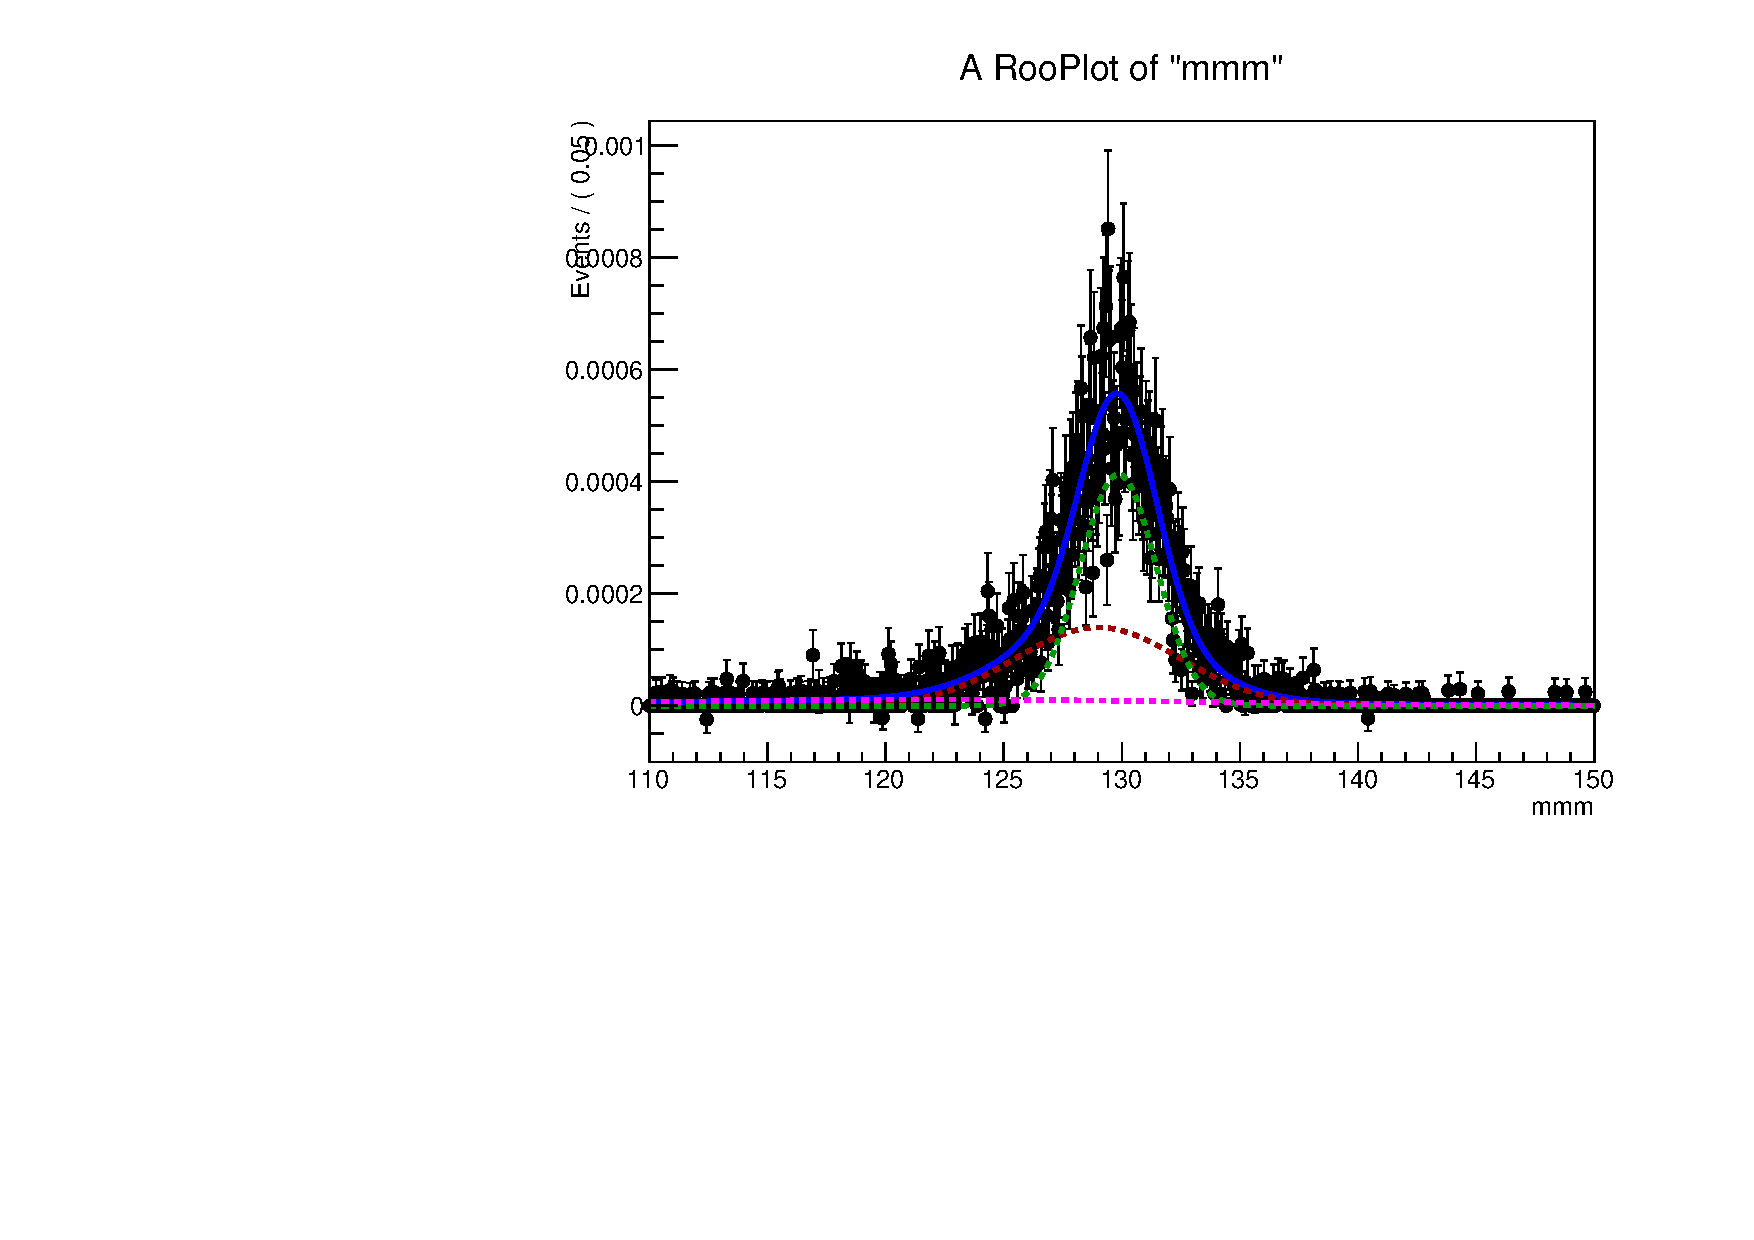
\includegraphics[width=.47\textwidth]{figures/signal_model/AppendixBdt/ZH/130/fit_mh_130_ZH_cat0.pdf}
}
 & \parbox{0.47\textwidth}{
\centering
{\bfseries fit-mh-130-ZH-cat1.pdf}
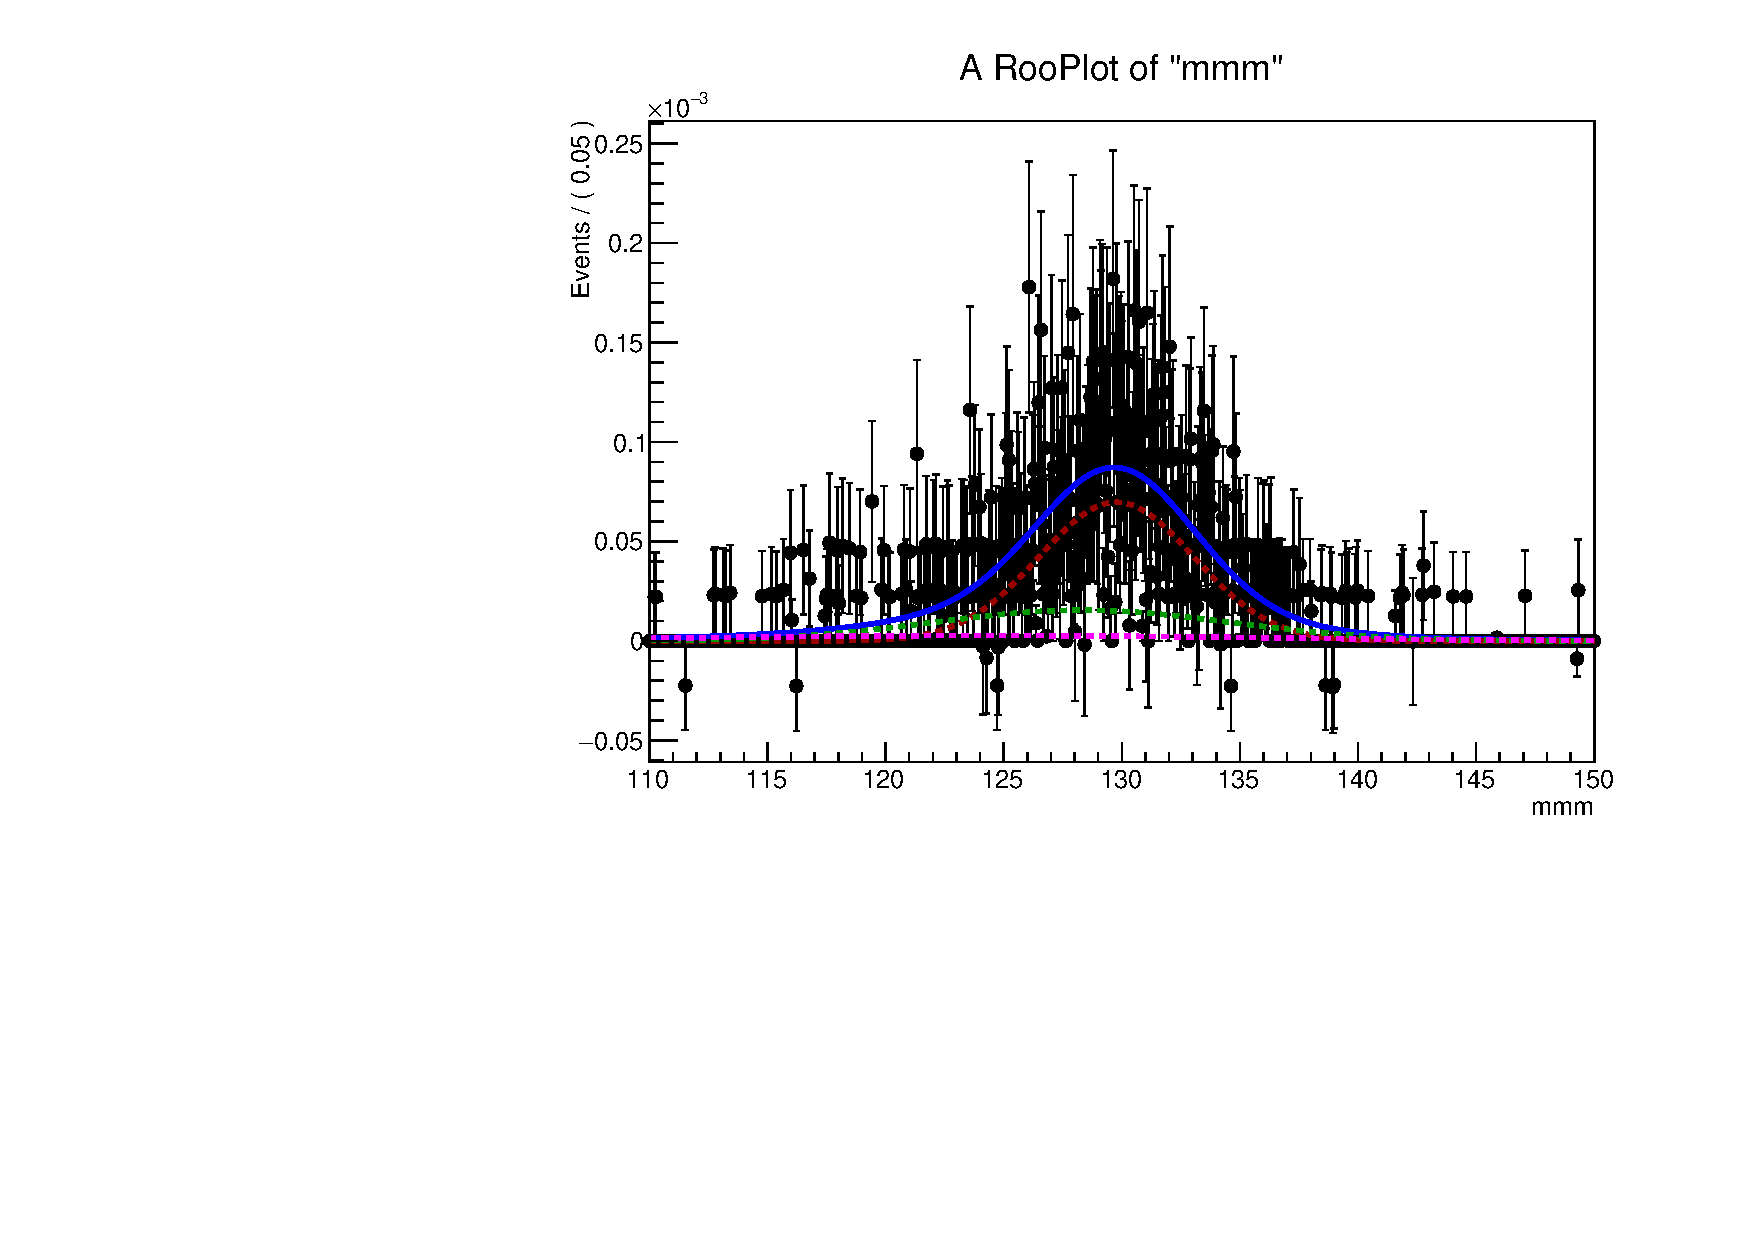
\includegraphics[width=.47\textwidth]{figures/signal_model/AppendixBdt/ZH/130/fit_mh_130_ZH_cat1.pdf}
}
 \\
\hline
\parbox{0.47\textwidth}{
\centering
{\bfseries fit-mh-130-ZH-cat2.pdf}
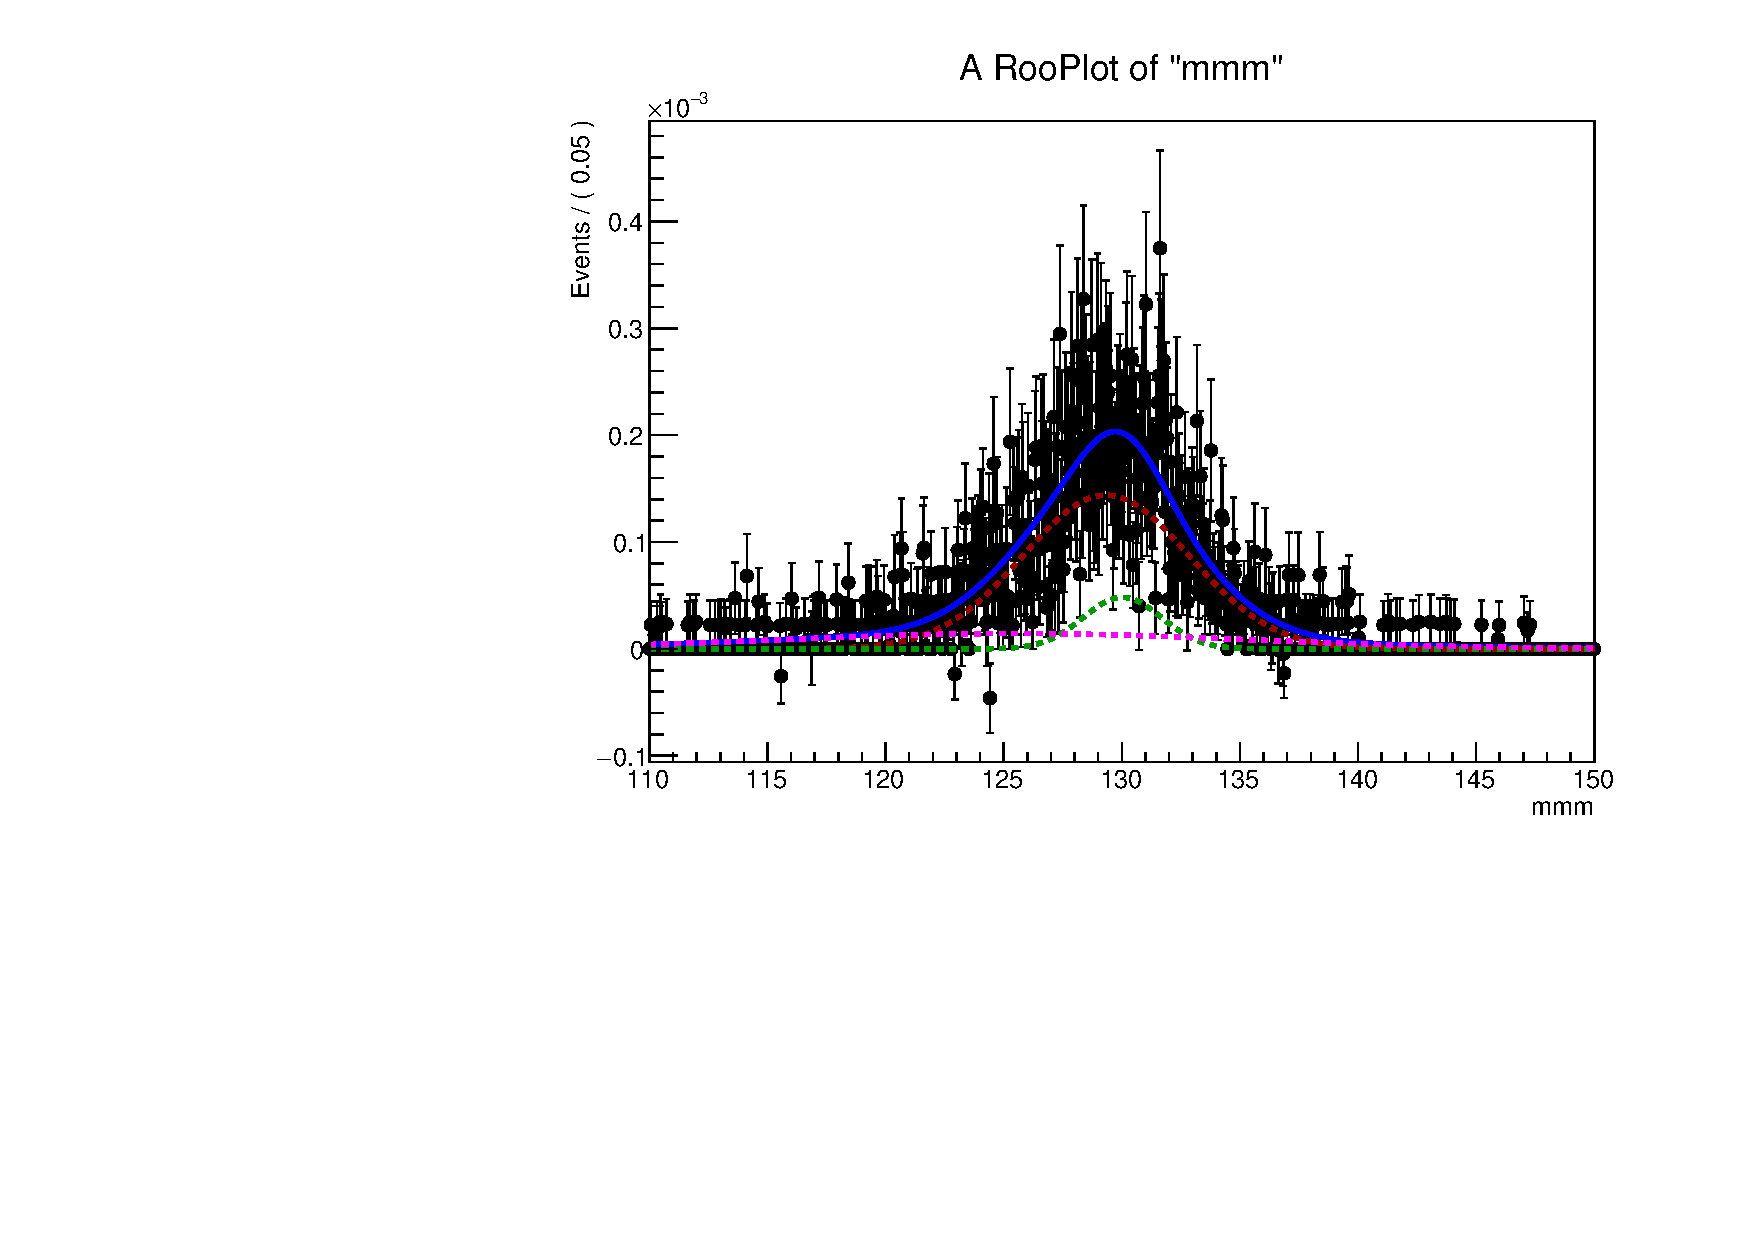
\includegraphics[width=.47\textwidth]{figures/signal_model/AppendixBdt/ZH/130/fit_mh_130_ZH_cat2.pdf}
}
 & \parbox{0.47\textwidth}{
\centering
{\bfseries fit-mh-130-ZH-cat3.pdf}
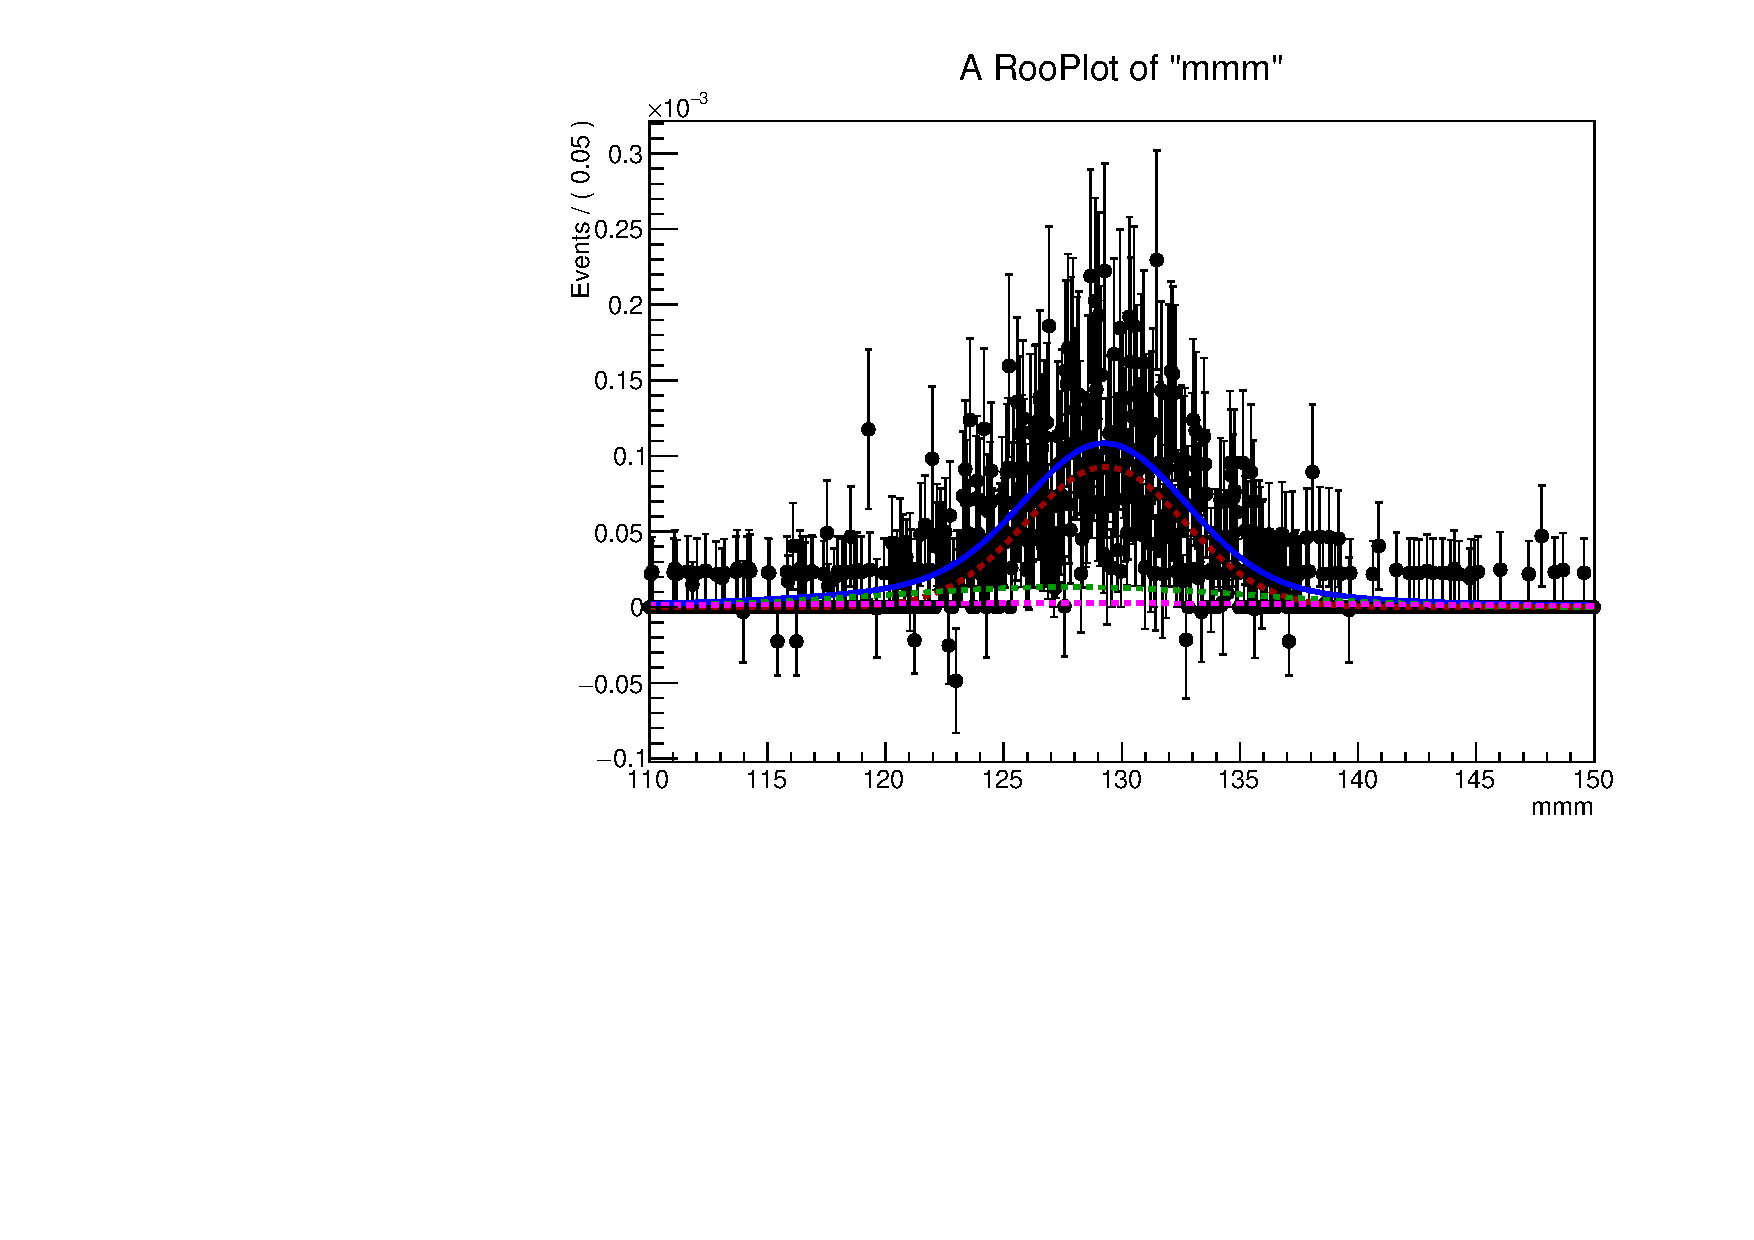
\includegraphics[width=.47\textwidth]{figures/signal_model/AppendixBdt/ZH/130/fit_mh_130_ZH_cat3.pdf}
}
 \\
\hline
\parbox{0.47\textwidth}{
\centering
{\bfseries fit-mh-130-ZH-cat4.pdf}
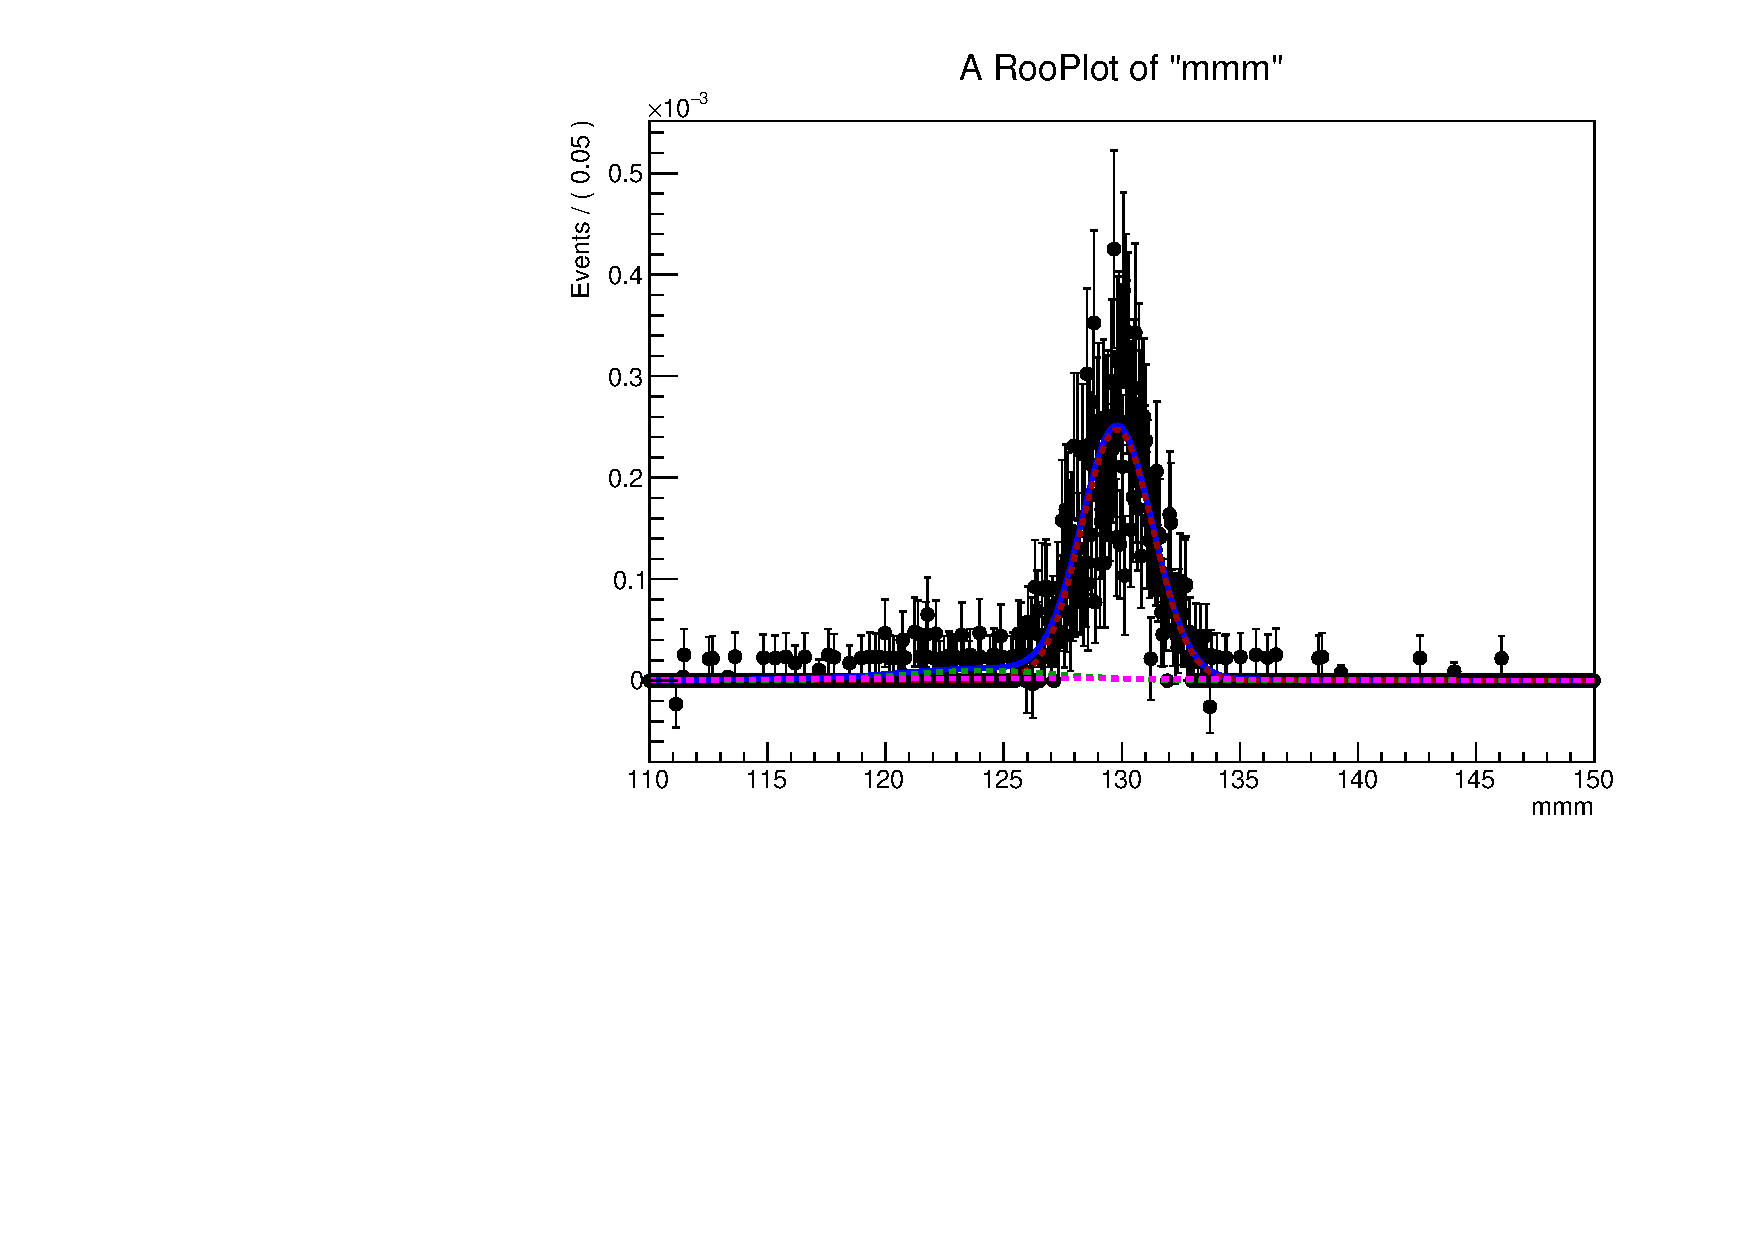
\includegraphics[width=.47\textwidth]{figures/signal_model/AppendixBdt/ZH/130/fit_mh_130_ZH_cat4.pdf}
}
 & \parbox{0.47\textwidth}{
\centering
{\bfseries fit-mh-130-ZH-cat5.pdf}
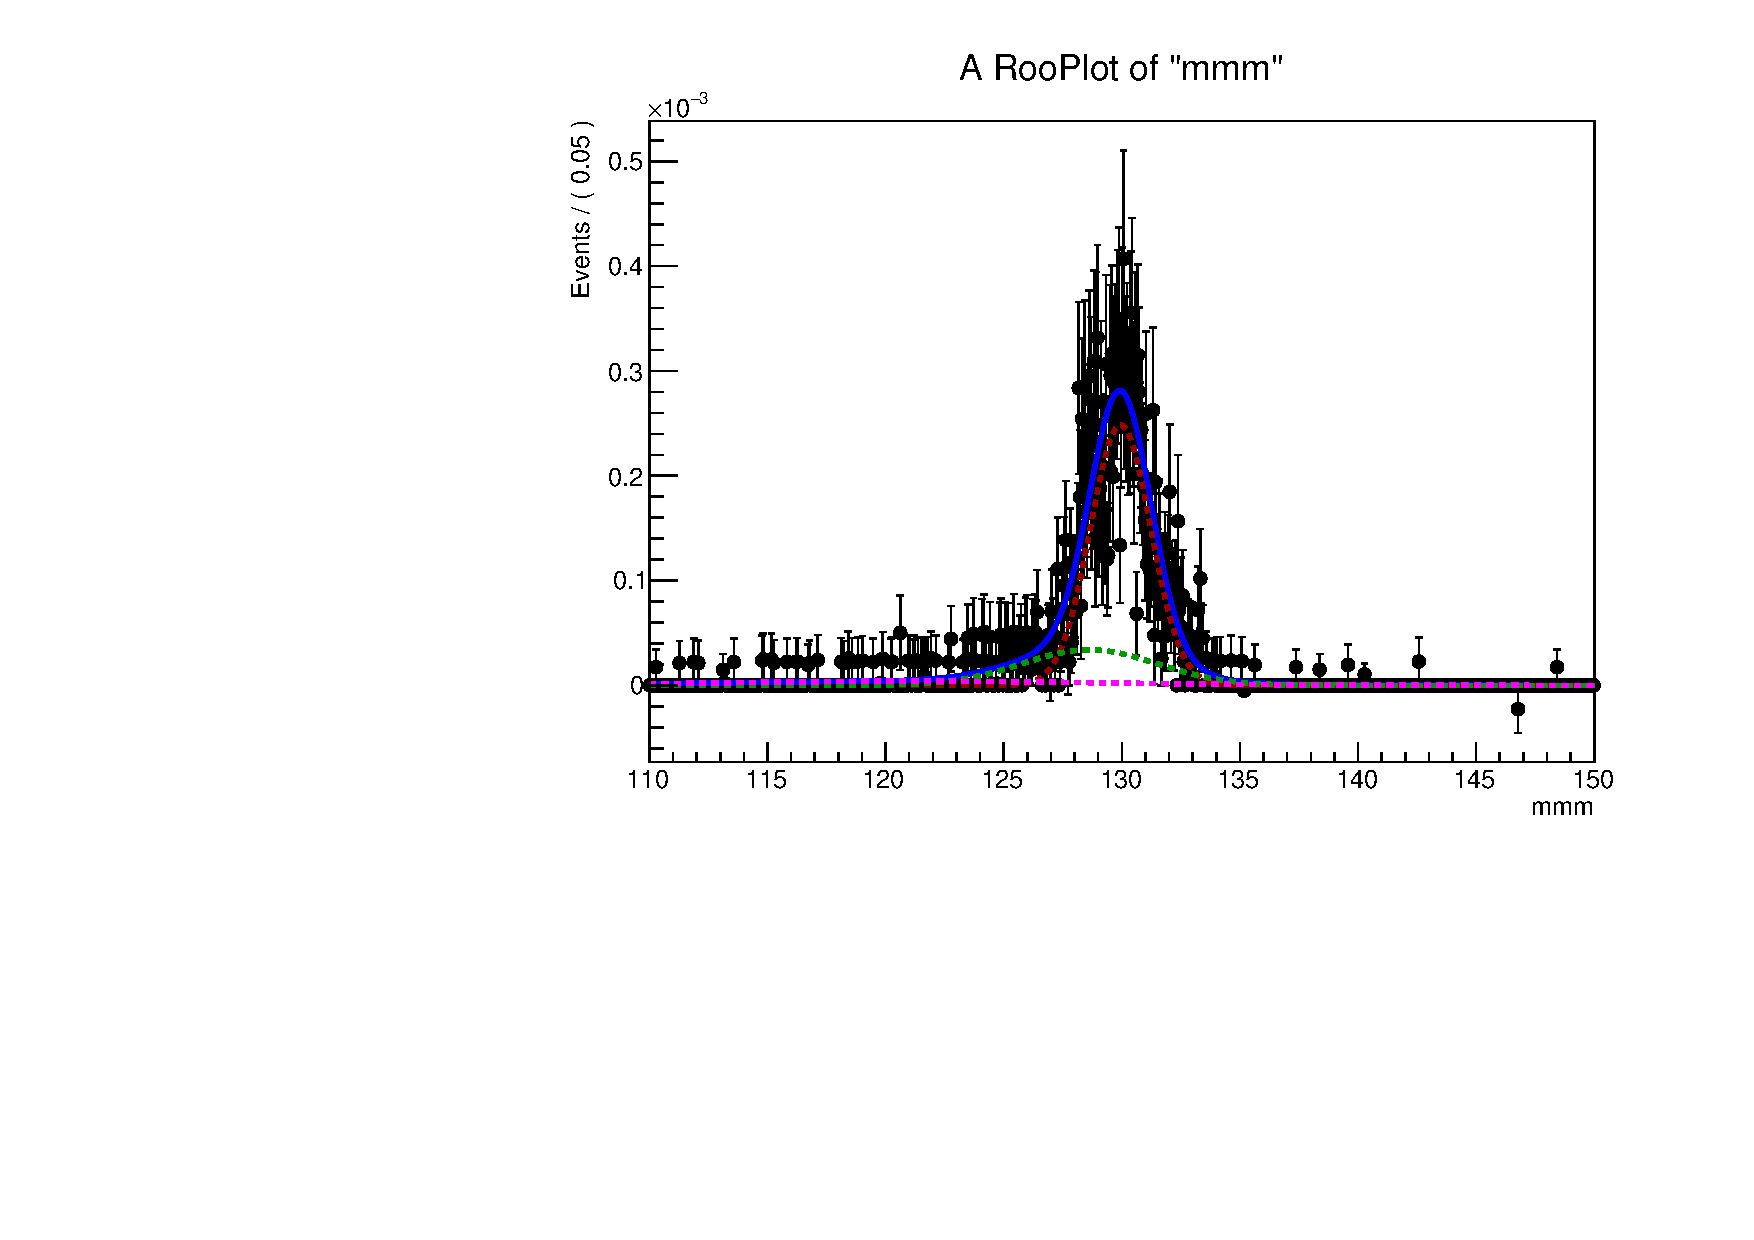
\includegraphics[width=.47\textwidth]{figures/signal_model/AppendixBdt/ZH/130/fit_mh_130_ZH_cat5.pdf}
}
 \\
\hline
\parbox{0.47\textwidth}{
\centering
{\bfseries fit-mh-130-ZH-cat6.pdf}
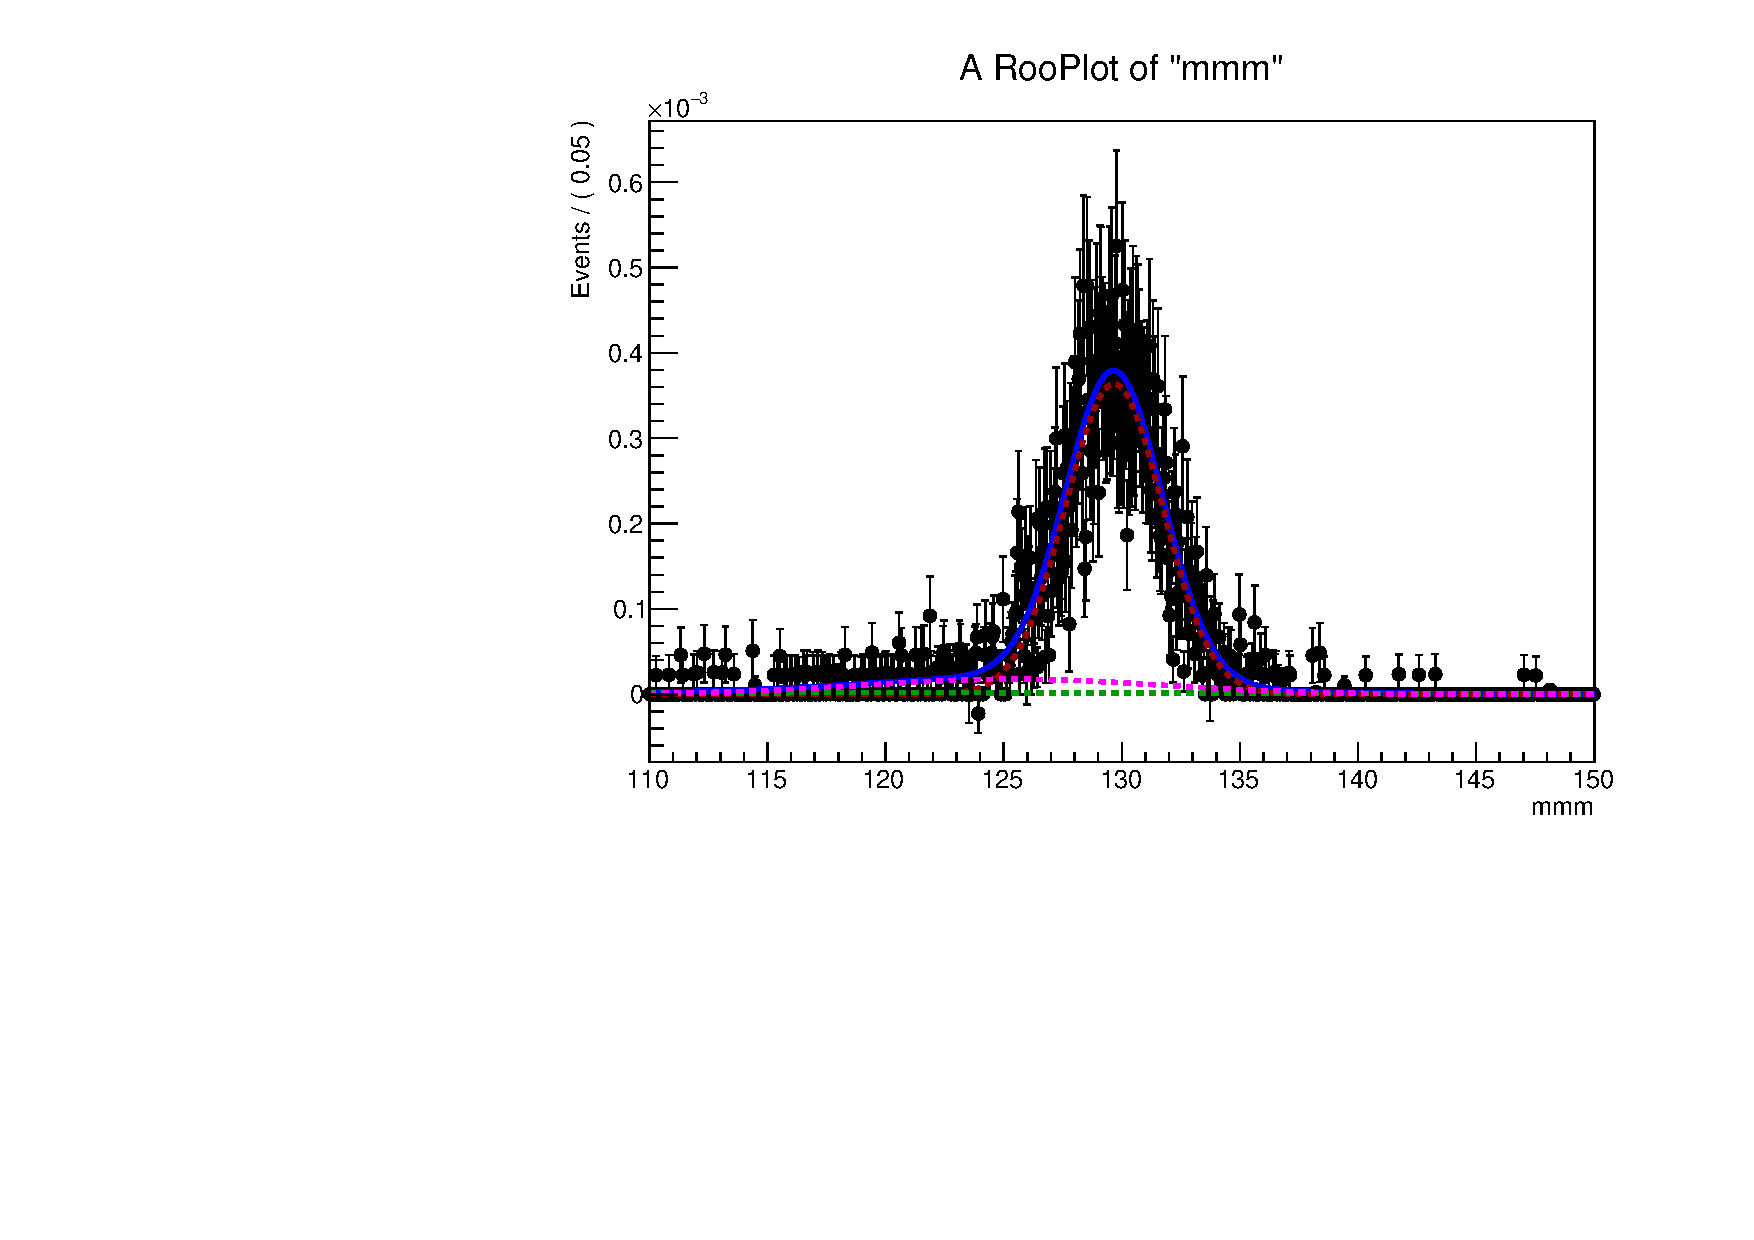
\includegraphics[width=.47\textwidth]{figures/signal_model/AppendixBdt/ZH/130/fit_mh_130_ZH_cat6.pdf}
}
 & \parbox{0.47\textwidth}{
\centering
{\bfseries fit-mh-130-ZH-cat7.pdf}
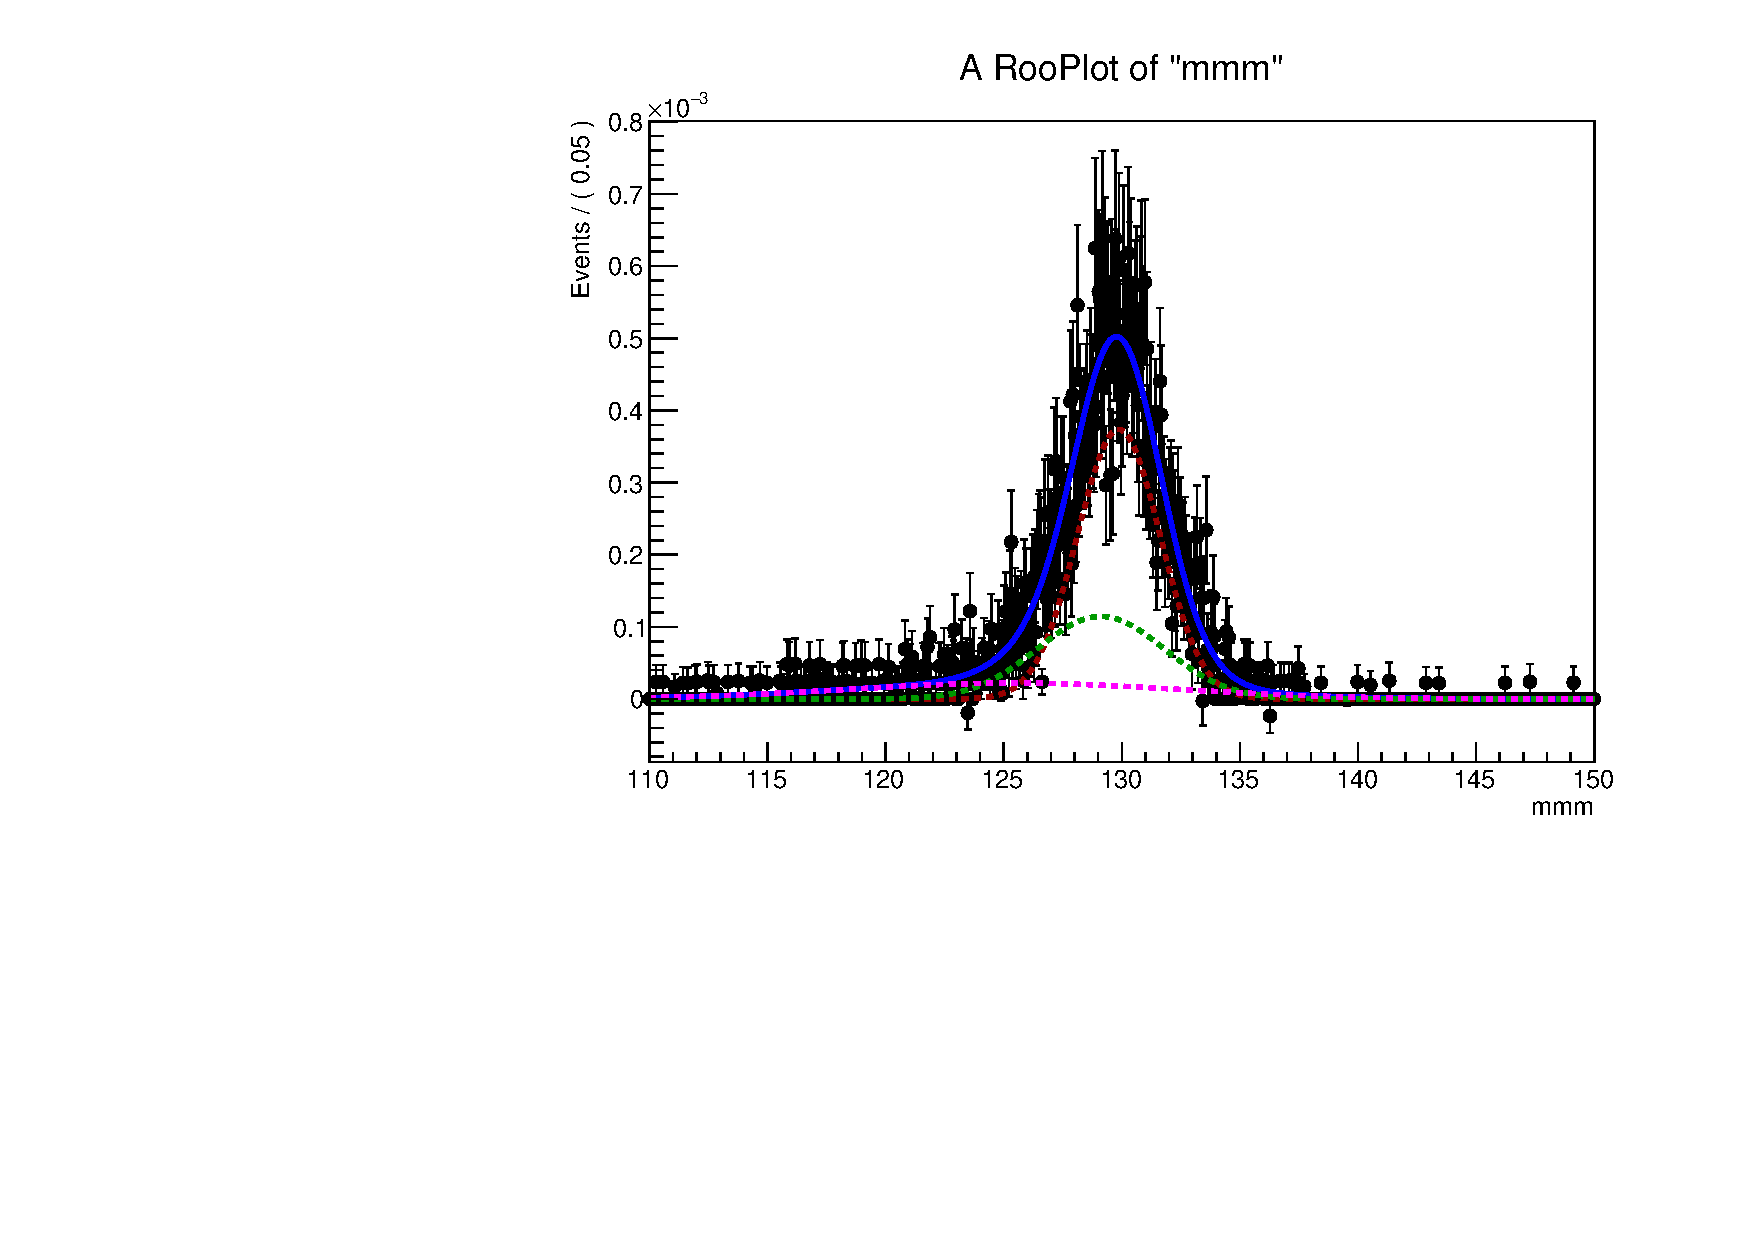
\includegraphics[width=.47\textwidth]{figures/signal_model/AppendixBdt/ZH/130/fit_mh_130_ZH_cat7.pdf}
}
 \\
\hline
\parbox{0.47\textwidth}{
\centering
{\bfseries fit-mh-130-ZH-cat8.pdf}
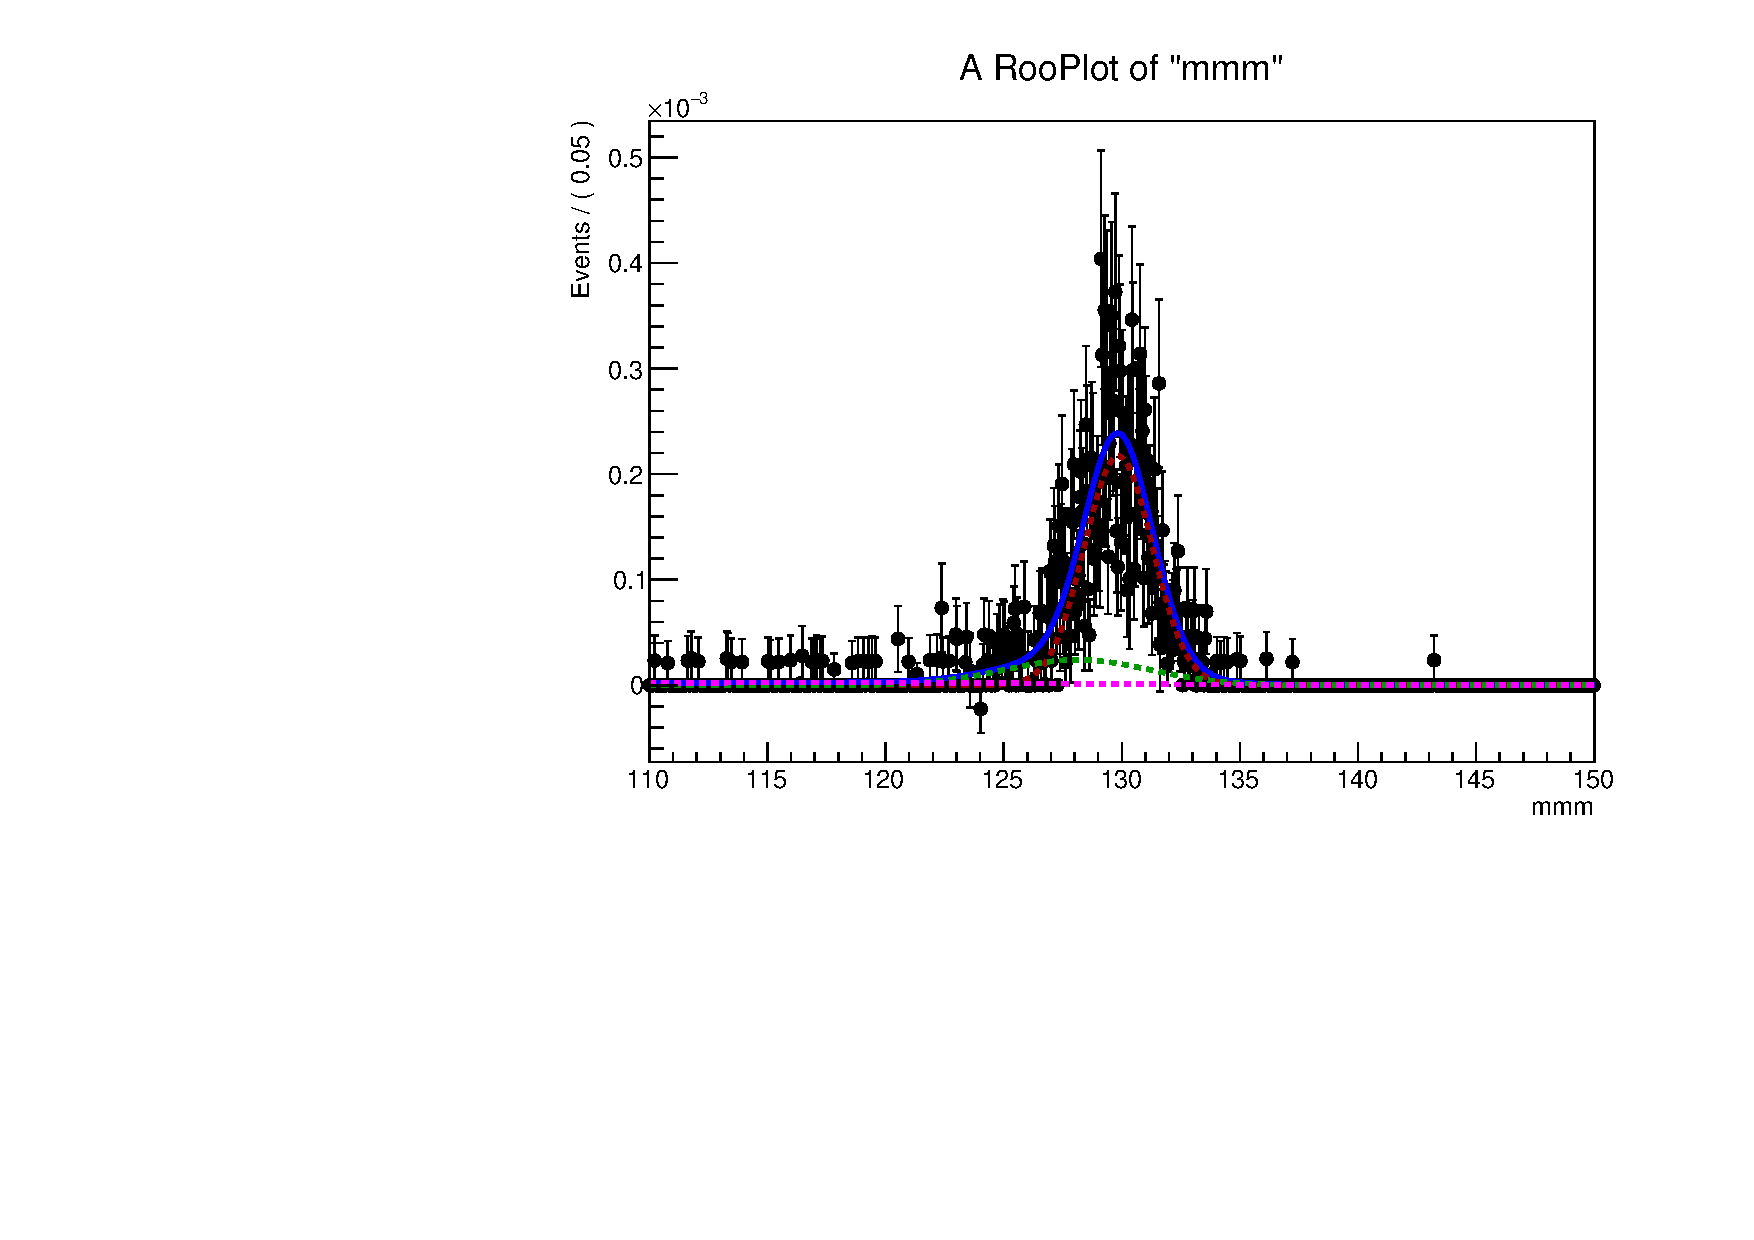
\includegraphics[width=.47\textwidth]{figures/signal_model/AppendixBdt/ZH/130/fit_mh_130_ZH_cat8.pdf}
}
 & \parbox{0.47\textwidth}{
\centering
{\bfseries fit-mh-130-ZH-cat9.pdf}
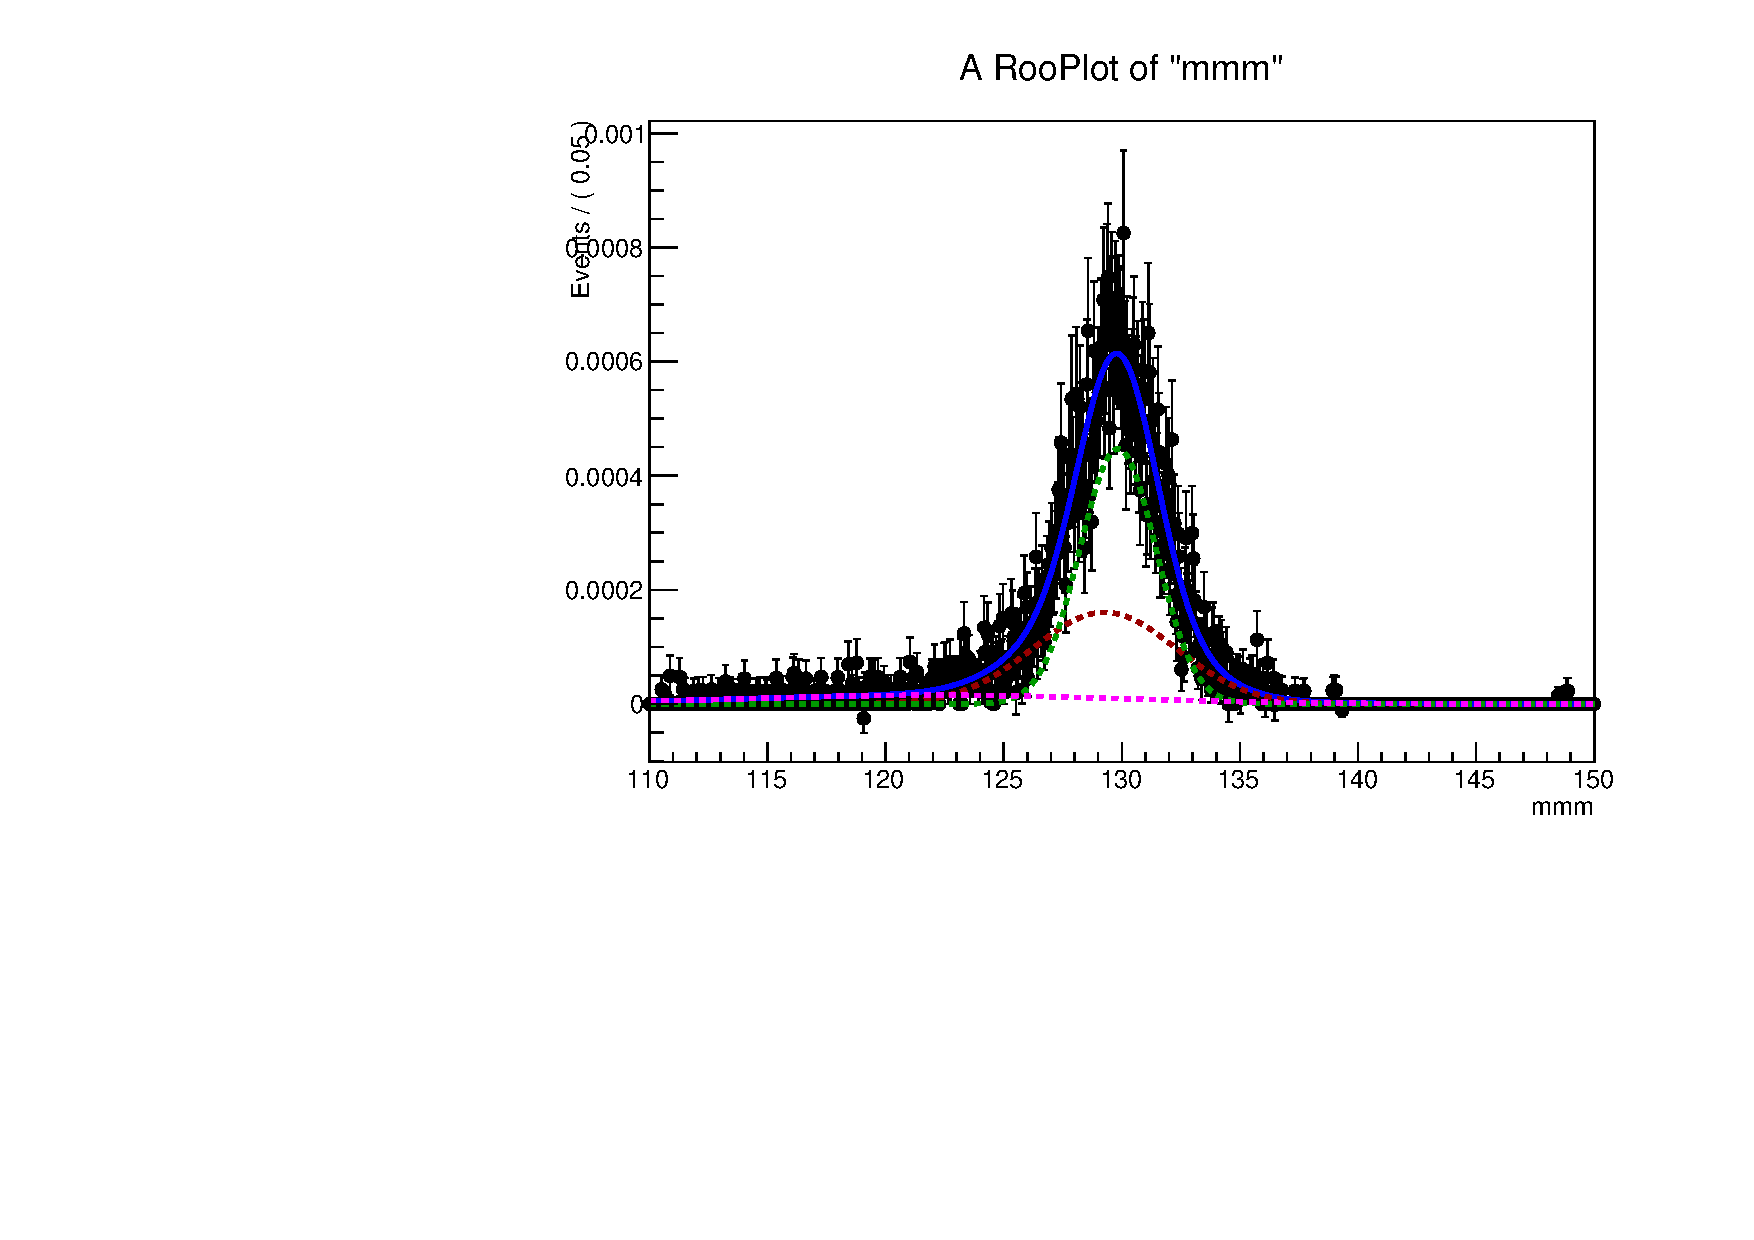
\includegraphics[width=.47\textwidth]{figures/signal_model/AppendixBdt/ZH/130/fit_mh_130_ZH_cat9.pdf}
}
 \\
\hline
\parbox{0.47\textwidth}{
\centering
{\bfseries fit-mh-130-ZH-cat10.pdf}
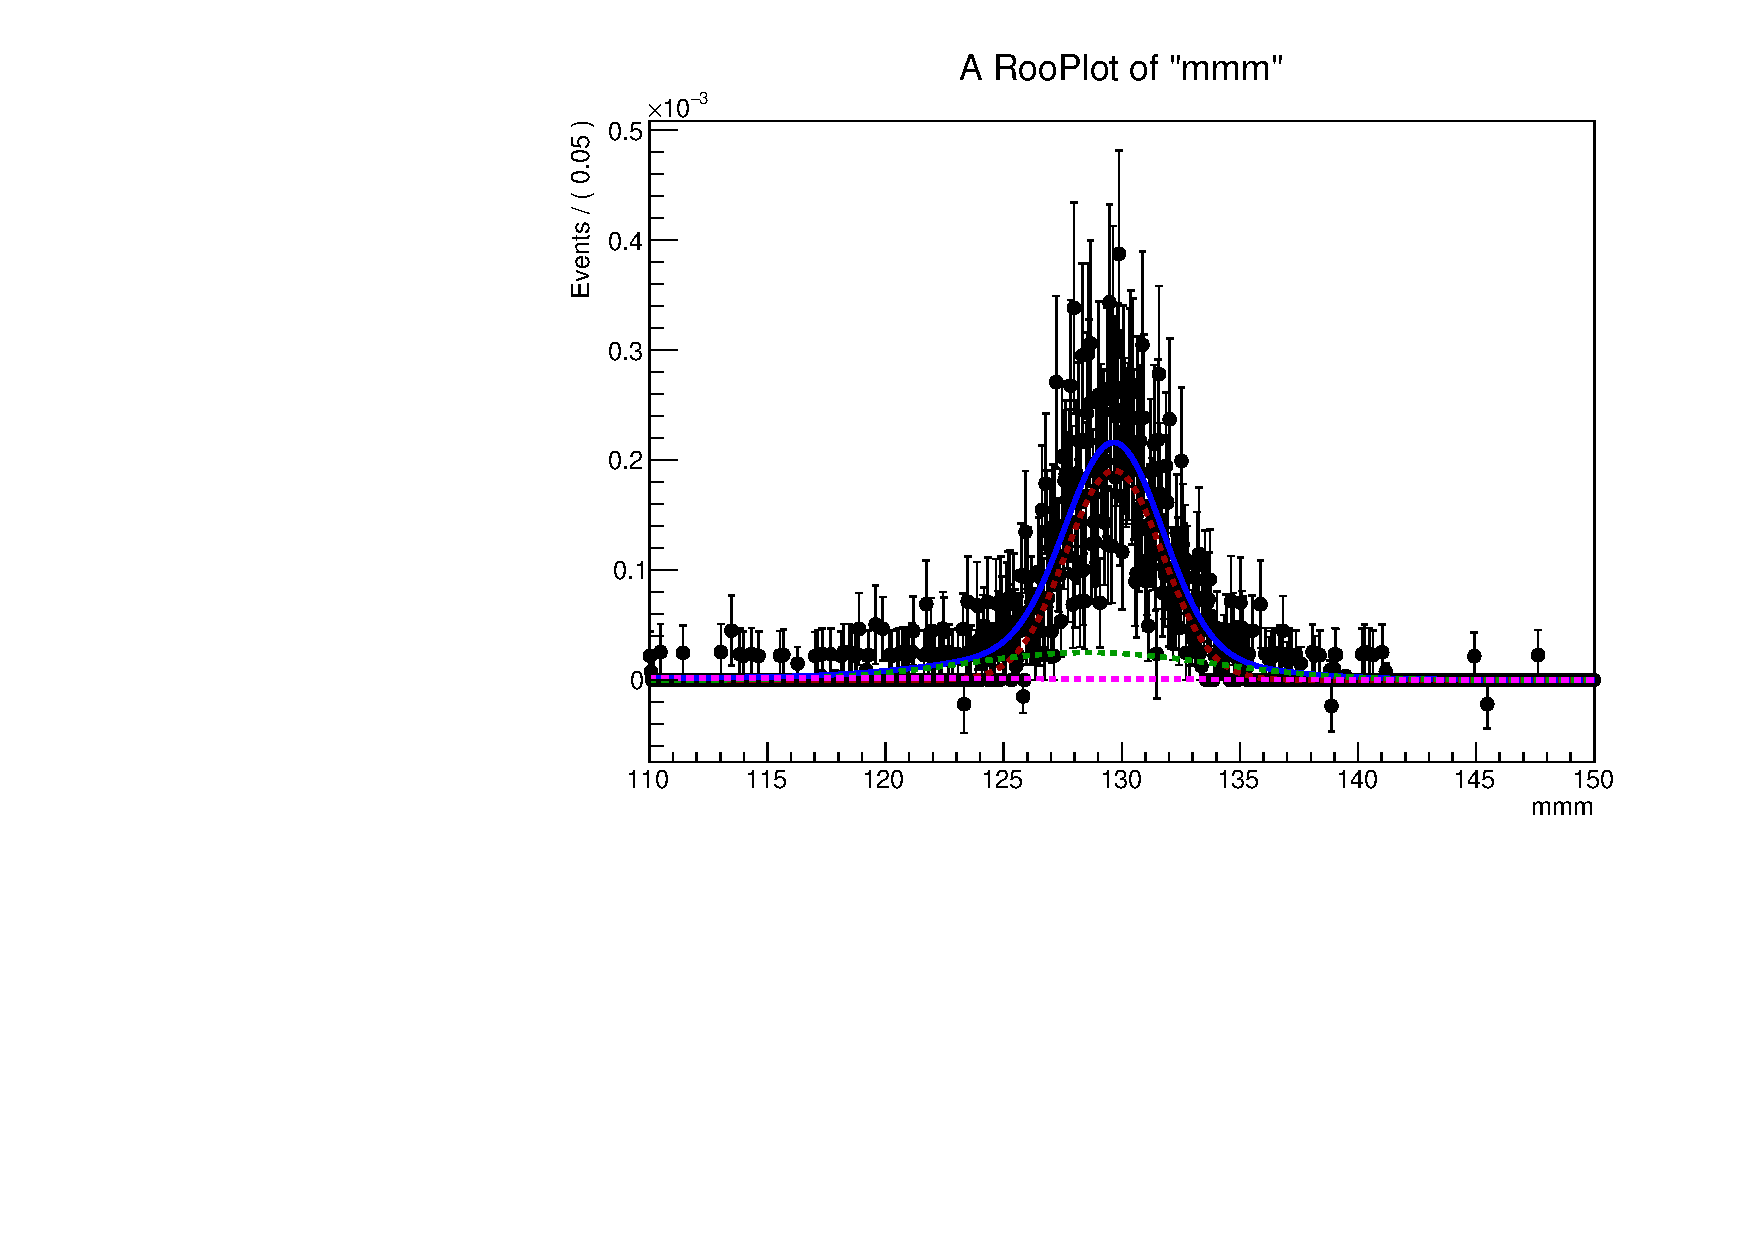
\includegraphics[width=.47\textwidth]{figures/signal_model/AppendixBdt/ZH/130/fit_mh_130_ZH_cat10.pdf}
}
 & \parbox{0.47\textwidth}{
\centering
{\bfseries fit-mh-130-ZH-cat11.pdf}
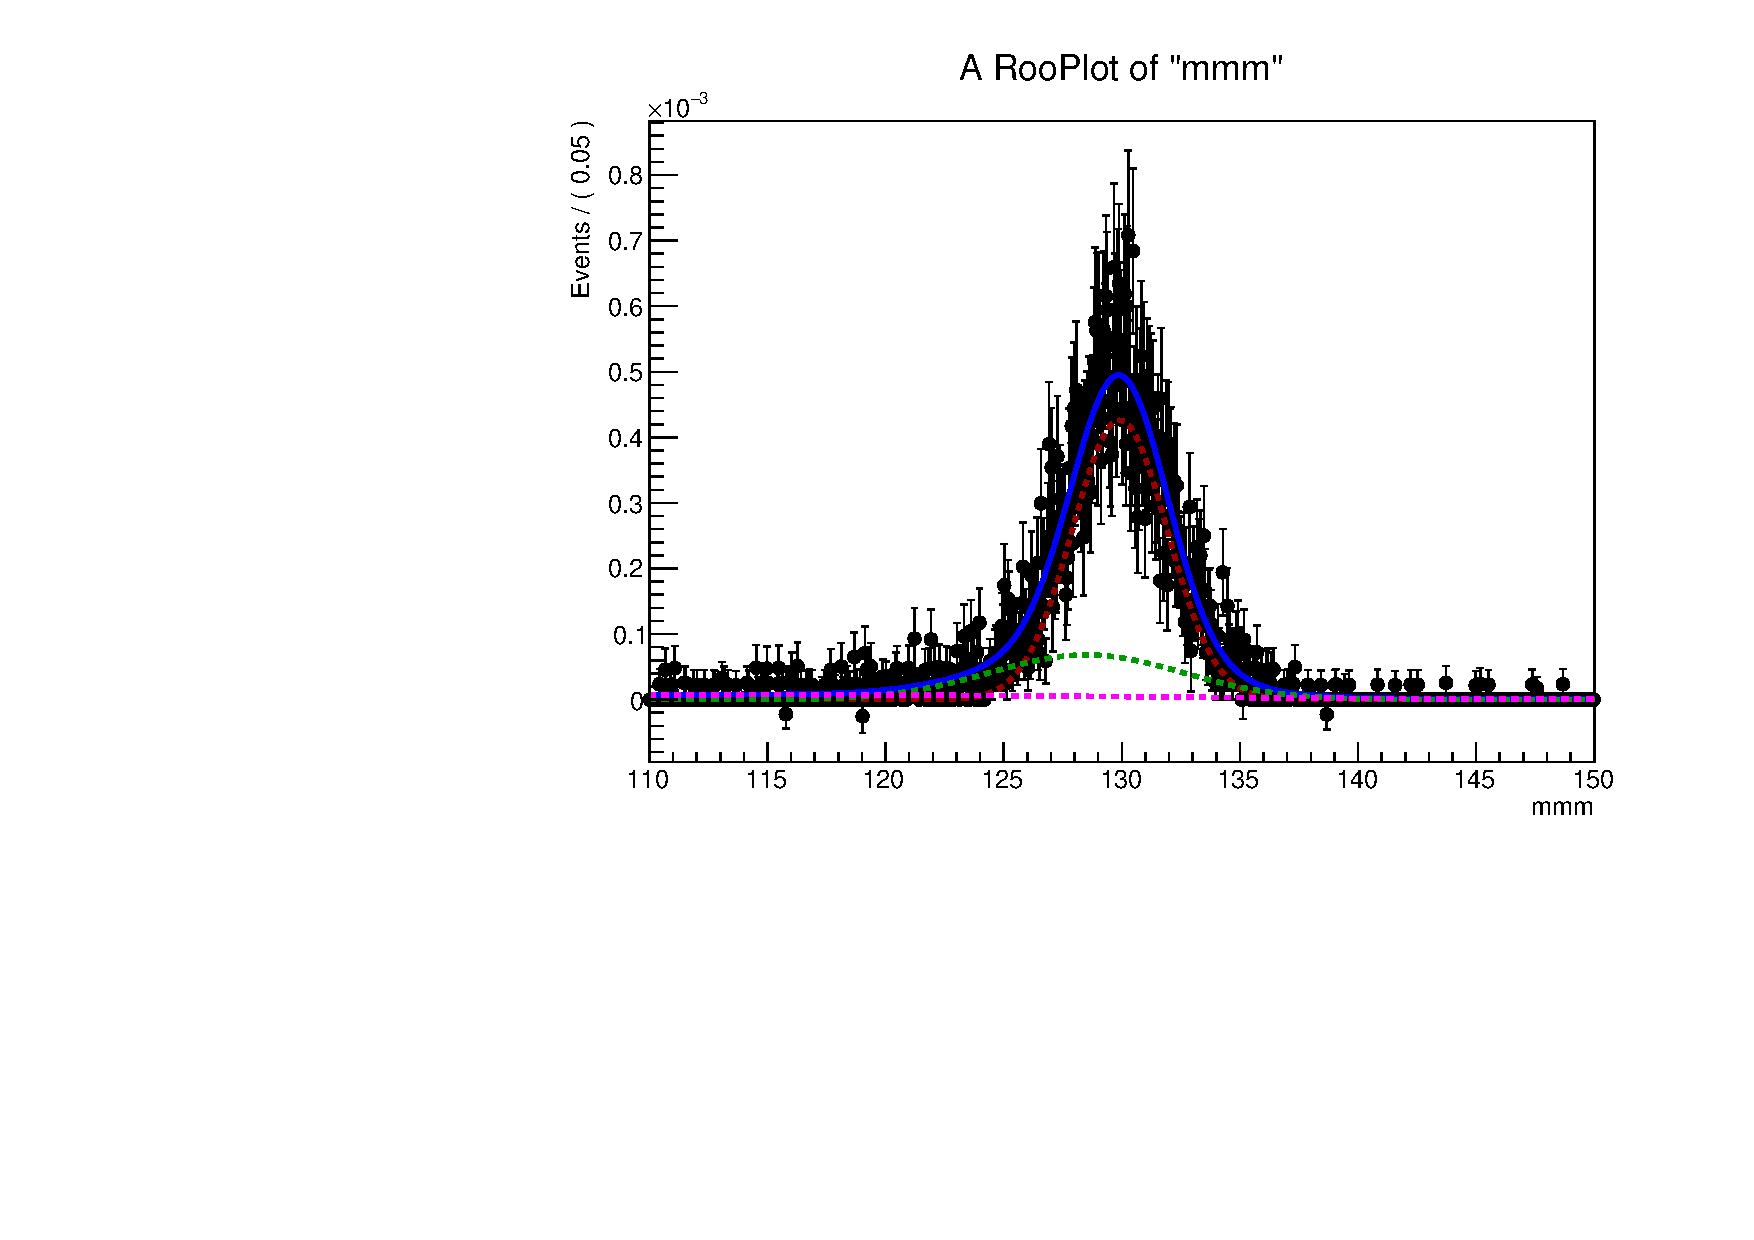
\includegraphics[width=.47\textwidth]{figures/signal_model/AppendixBdt/ZH/130/fit_mh_130_ZH_cat11.pdf}
}
 \\
\hline
\parbox{0.47\textwidth}{
\centering
{\bfseries fit-mh-130-ZH-cat12.pdf}
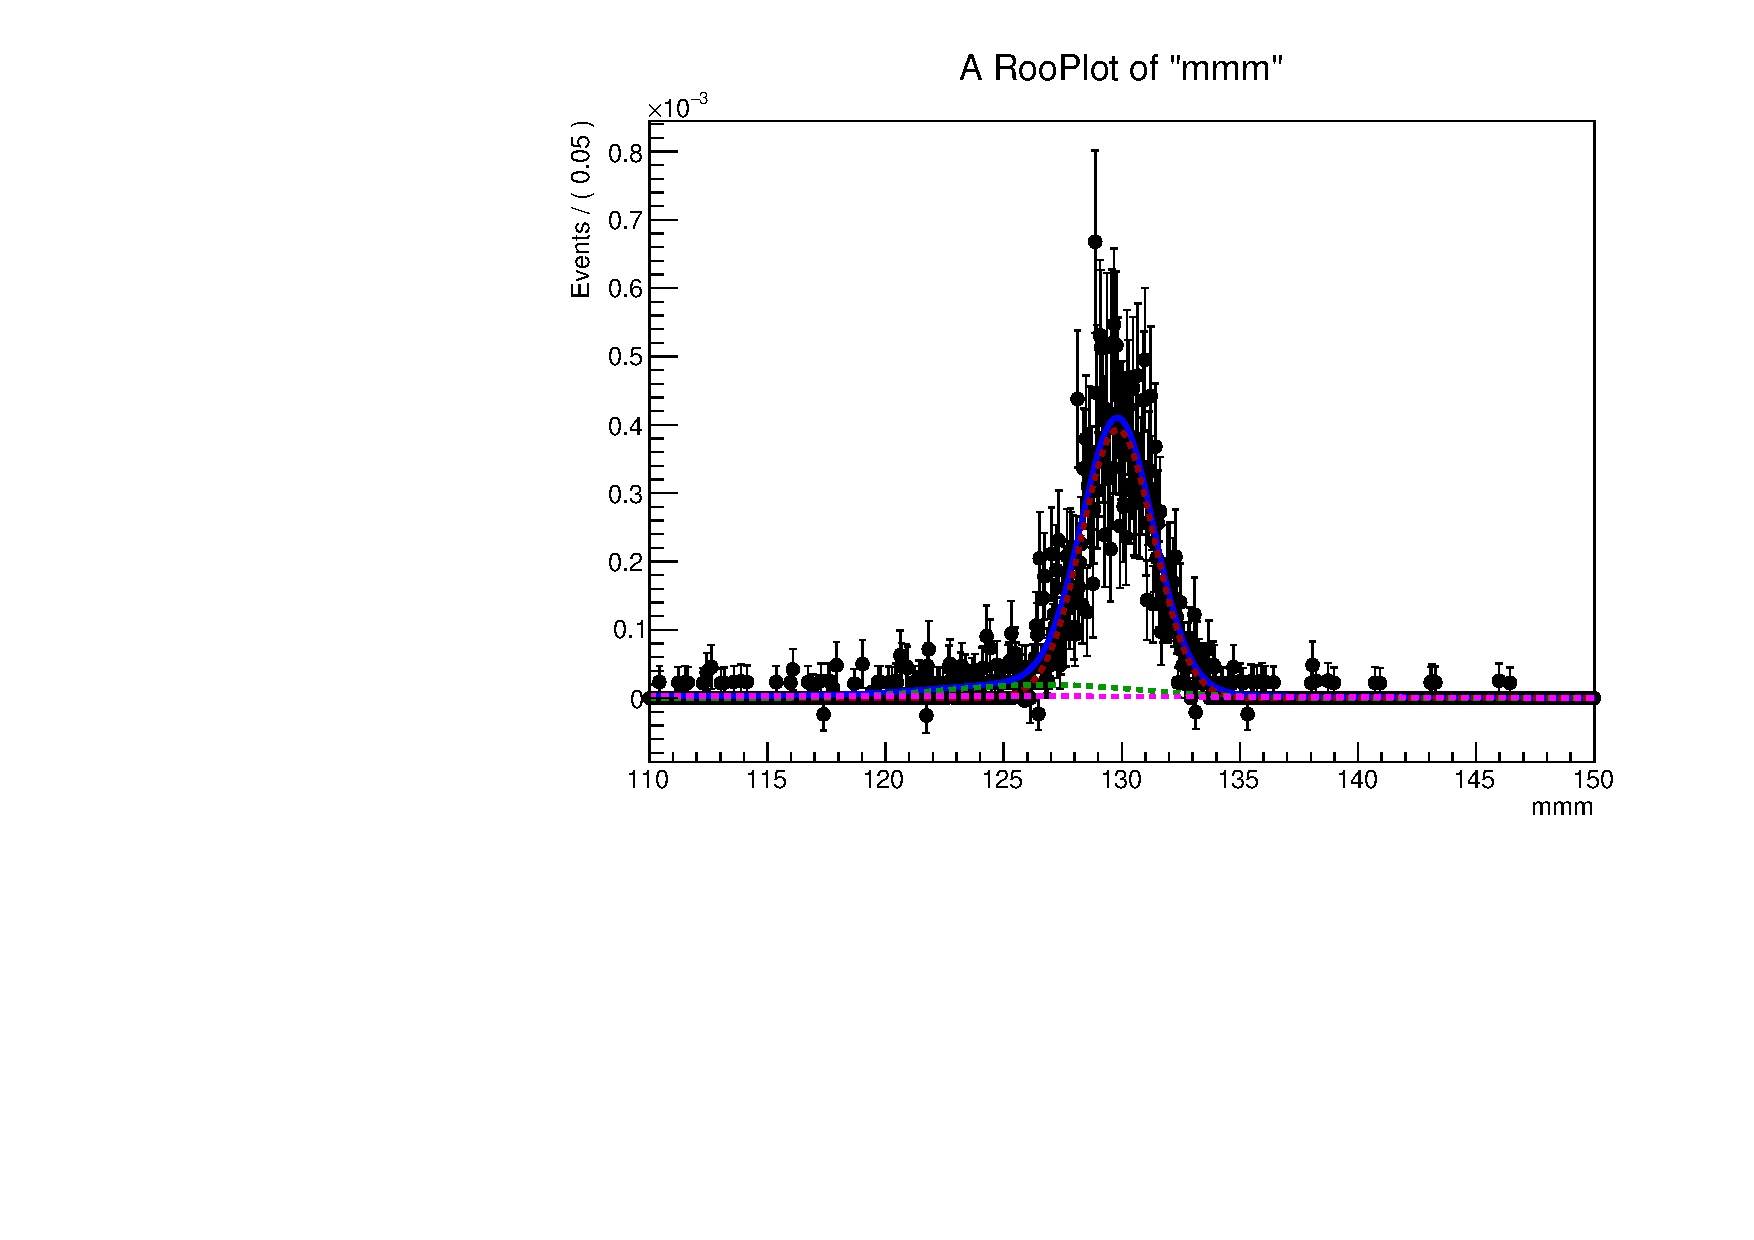
\includegraphics[width=.47\textwidth]{figures/signal_model/AppendixBdt/ZH/130/fit_mh_130_ZH_cat12.pdf}
}
 & \parbox{0.47\textwidth}{
\centering
{\bfseries fit-mh-130-ZH-cat13.pdf}
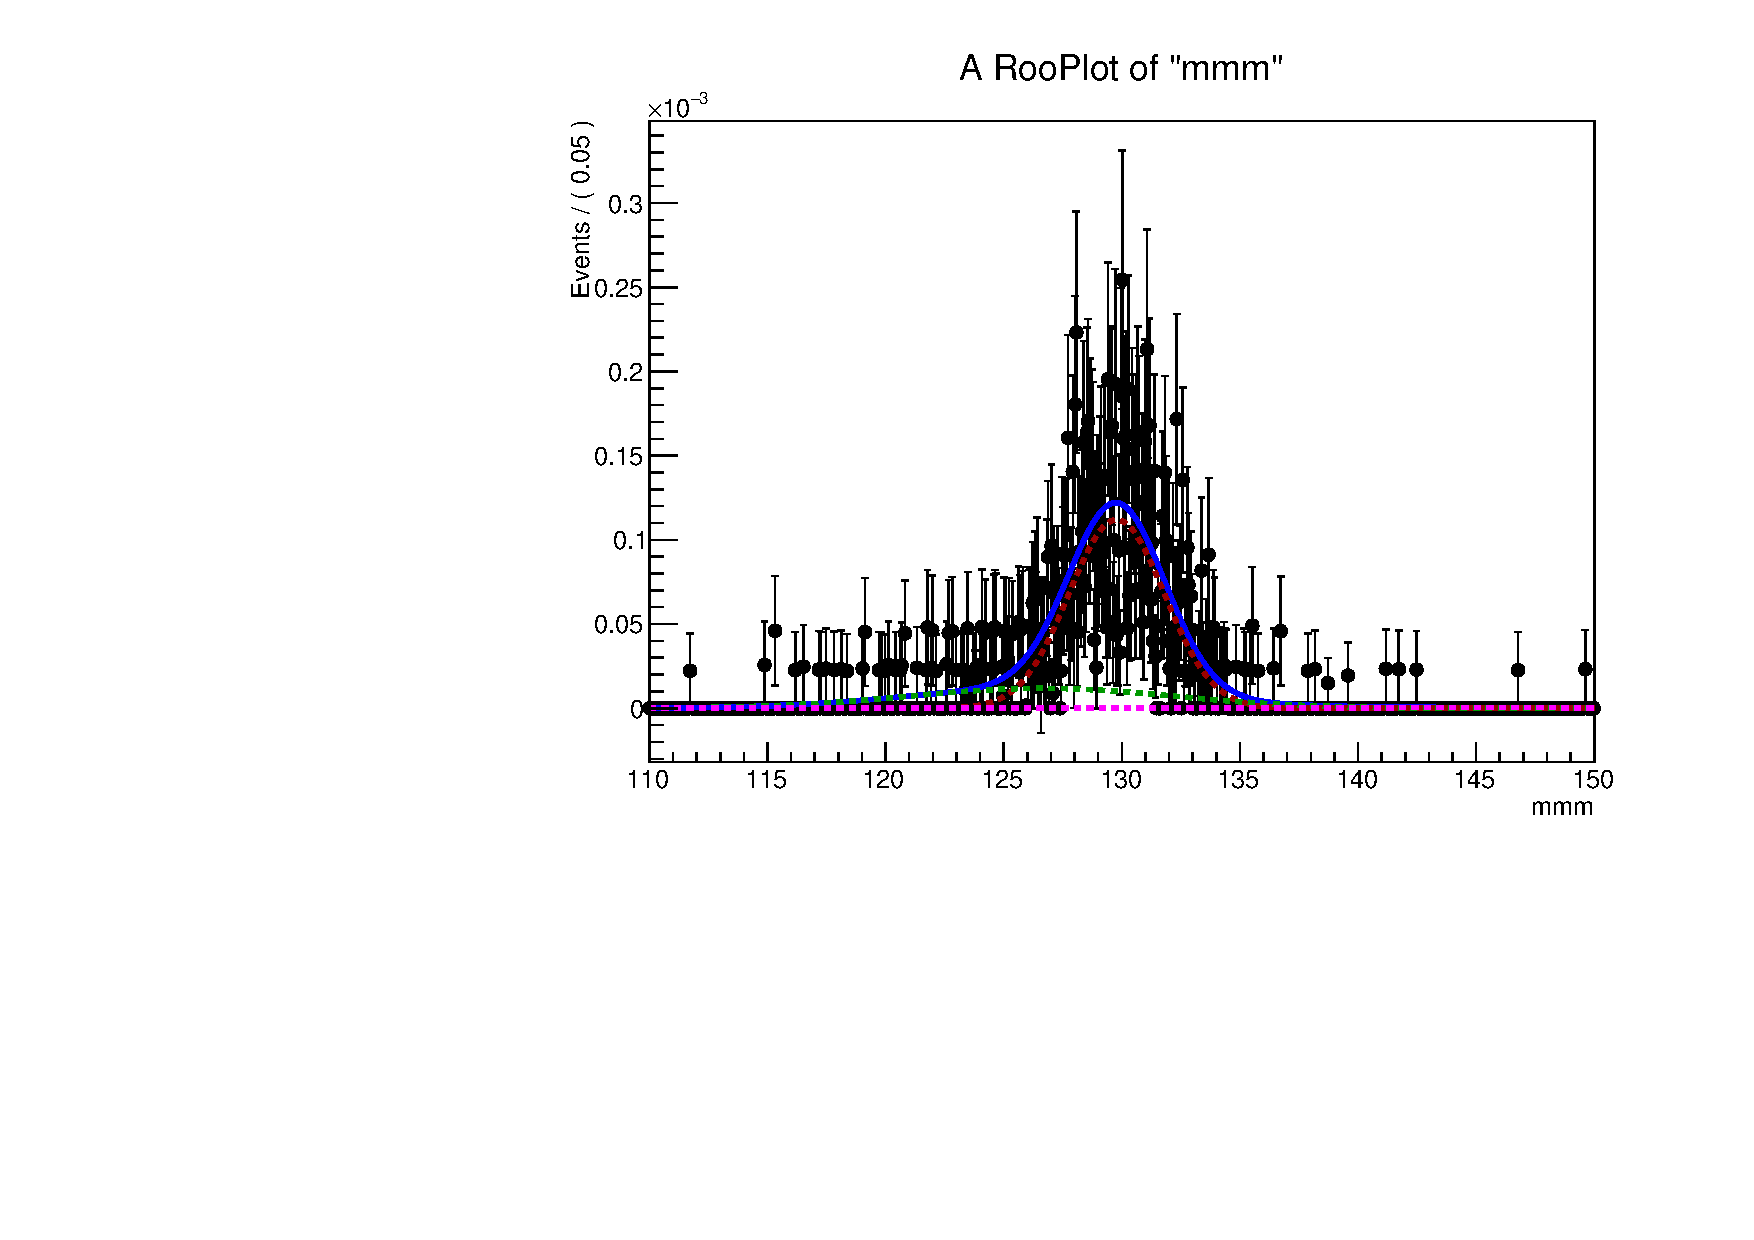
\includegraphics[width=.47\textwidth]{figures/signal_model/AppendixBdt/ZH/130/fit_mh_130_ZH_cat13.pdf}
}
 \\
\hline
\parbox{0.47\textwidth}{
\centering
{\bfseries fit-mh-130-ZH-cat14.pdf}
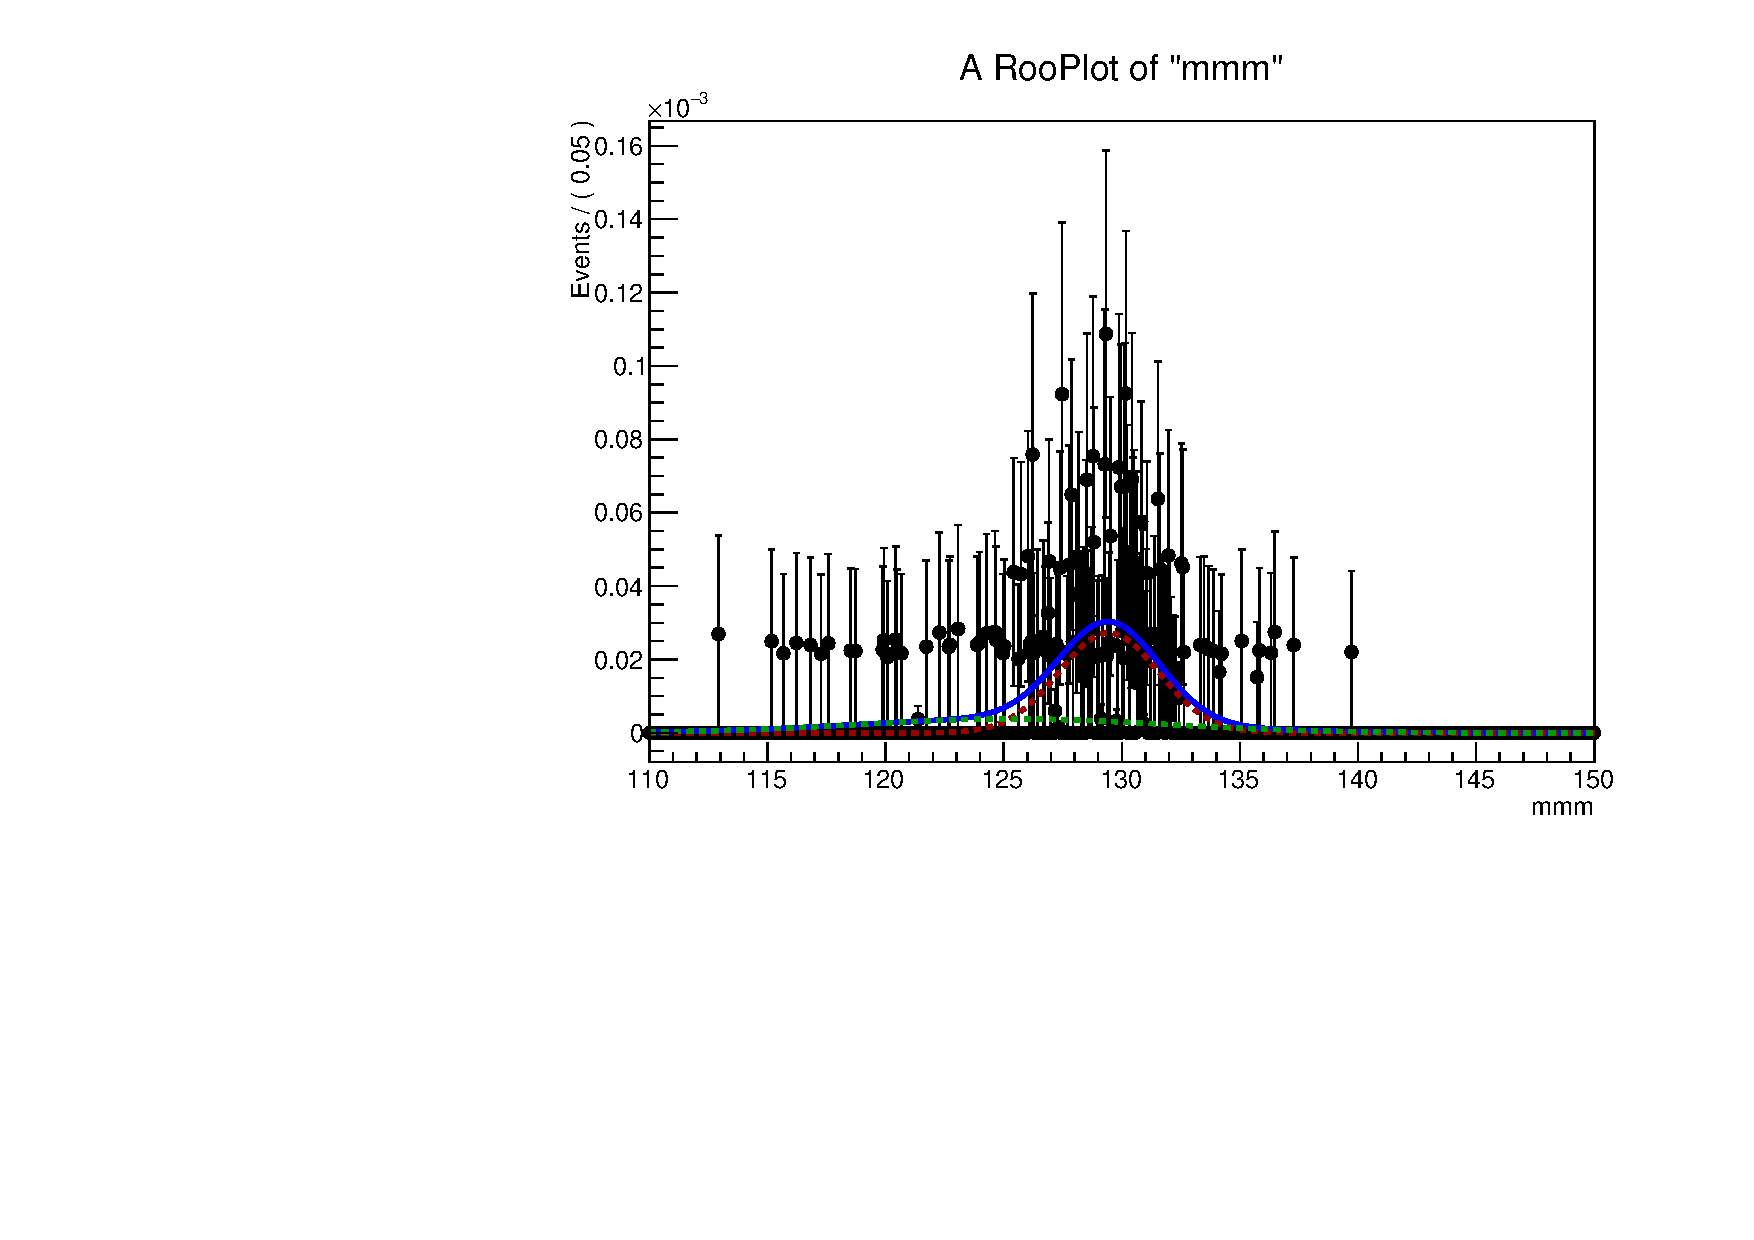
\includegraphics[width=.47\textwidth]{figures/signal_model/AppendixBdt/ZH/130/fit_mh_130_ZH_cat14.pdf}
}
 & \parbox{0.47\textwidth}{
\centering
{\bfseries fit-mh-130-ZH-cat15.pdf}
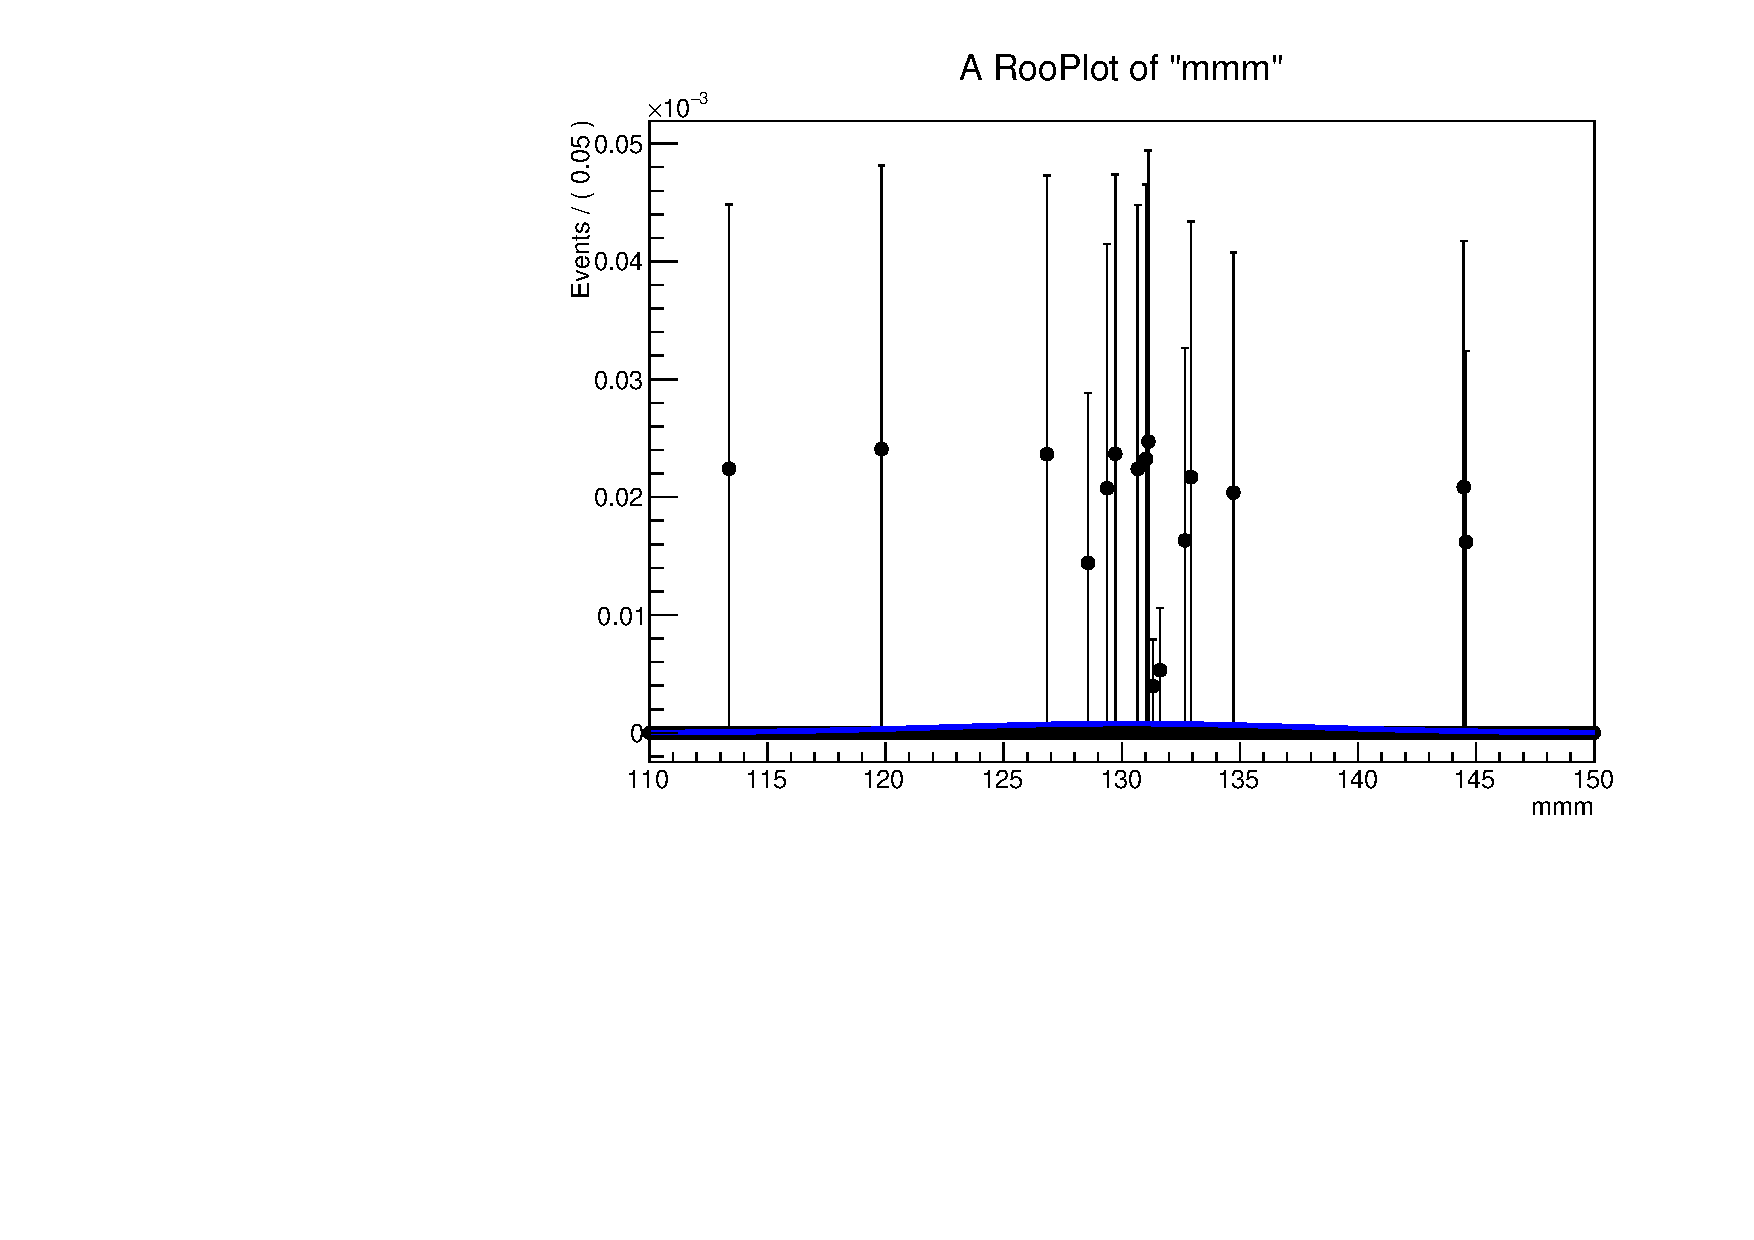
\includegraphics[width=.47\textwidth]{figures/signal_model/AppendixBdt/ZH/130/fit_mh_130_ZH_cat15.pdf}
}
 \\
\hline
\end{longtable}
